
Neste capítulo, serão apresentados os resultados obtidos a partir da aplicação do que foi proposto na seção~\ref{introducao:objetivos}, seguido de uma análise dos dados.

\section{Caracterização de redes}
\label{section:metricas-redes}

Neste capítulo, faremos uma caracterização dos dados a partir de diferentes modelagens utilizando redes complexas.

\subsection{Redes UF-UF}
\label{section:metricas-redes:uf}

Nesta seção, será apresentada a caracterização de uma rede entre unidades federativas brasileiras.

\begin{table}[htb]
\centering
\caption{Métricas do grafo de transações entre UFs}
\label{tab:metricas-redes:grafo-por-uf}
    \begin{tabular}{l|r}
    \toprule
    Métrica &  Valor \\
    \midrule
    Quantidade de nós         &  27      \\
    Quantidade de arestas     & 377      \\
    Diâmetro                  &   2      \\
    Raio                      &   1      \\
    Grau médio                &  26.9259 \\
    Densidade                 &   1.0740 \\
    Transitividade            &   0.9971 \\
    Assortatividade de grau   &  -0.0356 \\
    Assortatividade de região &  -0.0025 \\
    \bottomrule
    \end{tabular}
\fdadospesquisa
\end{table}

Essa rede foi montada utilizando os dados de transações entre janeiro de 2019 e dezembro de 2019. Cada vértice representa uma UF e cada aresta representa o valor total transacionado no período entre duas UFs. Nesta modelagem consideramos um grafo não-direcionado cíclico. Cada vértice possui um atributo chamado \textbf{região} indicando a região a que pertence aquela UF. Cada aresta além do atributo contendo o valor total transacional, e um atributo chamado \textbf{distância} correspondente ao inverso do valor total transacionado. Este atributo reflete a distância econômica entre dois vértices, uma vez que vértices que tenham um alto valor transacionado entre si terão uma relação mais próxima, o que pode ser útil na formulação de alguns algoritmos. A Tabela~\ref{tab:metricas-redes:grafo-por-uf} apresenta as métricas do grafo para esta modelagem.

\begin{table}[htb]
\centering
\caption{Métricas do grafo de transações entre UFs segmentadas por UF}
\label{tab:metricas-redes:grafo-por-uf-especificas1}
    \begin{tabular}{l|rrrrrr}
    \toprule
    UF & Grau & \shortstack{Coeficiente\\de agrupamento} &  \shortstack{Caminho mínimo\\ médio poderado} & \shortstack{Centralidade\\de informação} &  \shortstack{Centralidade\\de autovalor} &  \textit{PageRank} \\
    \midrule
    AC & 26 & 0.0003 & $2.61e^{-09}$ & $4.51e^{+07}$ & 0.0016 & 0.0077 \\
    AL & 27 & 0.0008 & $1.07e^{-09}$ & $1.15e^{+08}$ & 0.0057 & 0.0112 \\
    AM & 27 & 0.0045 & $5.06e^{-10}$ & $2.33e^{+08}$ & 0.0714 & 0.0468 \\
    AP & 26 & 0.0005 & $2.66e^{-09}$ & $5.57e^{+07}$ & 0.0016 & 0.0077 \\
    BA & 27 & 0.0030 & $5.27e^{-10}$ & $2.16e^{+08}$ & 0.0538 & 0.0348 \\
    CE & 27 & 0.0019 & $6.39e^{-10}$ & $1.81e^{+08}$ & 0.0199 & 0.0185 \\
    DF & 27 & 0.0015 & $5.74e^{-10}$ & $1.83e^{+08}$ & 0.0290 & 0.0162 \\
    ES & 27 & 0.0033 & $5.03e^{-10}$ & $2.24e^{+08}$ & 0.0801 & 0.0334 \\
    GO & 27 & 0.0037 & $5.17e^{-10}$ & $2.25e^{+08}$ & 0.0634 & 0.0401 \\
    MA & 27 & 0.0012 & $8.34e^{-10}$ & $1.46e^{+08}$ & 0.0093 & 0.0131 \\
    MG & 27 & 0.0054 & $4.82e^{-10}$ & $2.39e^{+08}$ & 0.1696 & 0.0744 \\
    MS & 27 & 0.0015 & $5.96e^{-10}$ & $1.75e^{+08}$ & 0.0249 & 0.0153 \\
    MT & 27 & 0.0019 & $6.21e^{-10}$ & $1.85e^{+08}$ & 0.0219 & 0.0204 \\
    PA & 27 & 0.0021 & $5.89e^{-10}$ & $1.90e^{+08}$ & 0.0261 & 0.0216 \\
    PB & 27 & 0.0014 & $7.46e^{-10}$ & $1.58e^{+08}$ & 0.0124 & 0.0140 \\
    PE & 27 & 0.0029 & $5.59e^{-10}$ & $2.14e^{+08}$ & 0.0339 & 0.0325 \\
    PI & 27 & 0.0007 & $1.37e^{-09}$ & $9.40e^{+07}$ & 0.0039 & 0.0084 \\
    PR & 27 & 0.0049 & $4.85e^{-10}$ & $2.37e^{+08}$ & 0.1416 & 0.0630 \\
    RJ & 27 & 0.0051 & $4.82e^{-10}$ & $2.38e^{+08}$ & 0.1596 & 0.0659 \\
    RN & 27 & 0.0011 & $8.10e^{-10}$ & $1.33e^{+08}$ & 0.0097 & 0.0125 \\
    RO & 27 & 0.0010 & $8.09e^{-10}$ & $1.45e^{+08}$ & 0.0100 & 0.0138 \\
    RR & 27 & 0.0003 & $1.83e^{-09}$ & $4.51e^{+07}$ & 0.0009 & 0.0067 \\
    RS & 27 & 0.0038 & $5.16e^{-10}$ & $2.26e^{+08}$ & 0.0680 & 0.0416 \\
    SC & 27 & 0.0042 & $4.97e^{-10}$ & $2.31e^{+08}$ & 0.0971 & 0.0474 \\
    SE & 27 & 0.0006 & $1.64e^{-09}$ & $9.23e^{+07}$ & 0.0025 & 0.0091 \\
    SP & 27 & 0.0119 & $4.59e^{-10}$ & $2.52e^{+08}$ & 0.9426 & 0.3101 \\
    TO & 27 & 0.0011 & $8.96e^{-10}$ & $1.42e^{+08}$ & 0.0085 & 0.0127 \\
    \bottomrule
    \end{tabular}
\fdadospesquisa
\end{table}

É possível notar que o grafo entre UFs é quase completo, com alto grau médio, refletindo o baixo diâmetro e raio da rede. Dado que estamos usando uma modelagem cíclica, aceitando arestas que conectam um vértice a ele mesmo, a densidade desta rede é maior que $1.0$. Temos também alta transitividade, e baixa assortatividade de grau e de região. Por ser um grafo bastante completo, é difícil tomar qualquer conclusão a partir destas métricas uma vez que elas irão refletir a simplicidade da topologia desta rede.

A Tabela~\ref{tab:metricas-redes:grafo-por-cnae-especificas1} nos dá uma ideia melhor da topologia do grafo. Para essas métricas agora consideramos a formulação usando arestas ponderadas pelo valor total transacionado pelas UFs. Para os caminhos mínimos, foi utilizada a distância entre UFs, como definido anteriormente.

Todos as UFs estão conectadas entre si com uma exceção: o estado do Acre não possui conexão com o estado do Amapá. O estado de Sâo Paulo se sobressai com maiores valores de coeficiente de agrupamento, centralidade de autovalor, e pagerank por ter um maior valor transacionado entre este estado e todos os outros se comparado aos demais, algo que já foi descrito na seção~\ref{chapter:impacto-economico}. Observando outros estados da região sudeste, como Rio de Janeiro de Minas Gerais, estes também tem valores importantes para essas métricas mostrando sua importância, novamente refletindo a tendência dessa região de se sobressair quanto ao valor transacionado e influenciando positivamente nestas métricas. Os estados da região norte, como Acre, Amapá, e Roraima apresentaram baixos valores para estas métricas refletindo os baixos valores transacionados por estas UFs com as demais. Sendo assim, apesar de uma topologia simples, ela se mostra razoavelmente eficaz em mostrar a importância de cada estado em relação às relações econômicas entre UFs brasileiras, também obedecendo às limitações e ao viés desta base de dados.

Nesta análise, não consideramos as métricas de centralidade de intermediação, caminho mínimo médio, e excentricidade, uma vez que o grafo é quase completo e essas medidas refletiriam apenas o grau de cada vértice, apresentando pouca variância e sendo redundante com o restando dos dados obtidos.

\subsection{Redes Seção-Seção}
\label{section:metricas-redes:secao}

Nesta seção, será apresentada a caracterização de uma rede entre seções de CNAE.

\begin{table}[htb]
\centering
\caption{Métricas do grafo de transações entre seções}
\label{tab:metricas-redes:grafo-por-secao}
    \begin{tabular}{l|r}
    \toprule
    Métrica &  Valor \\
    \midrule
    Quantidade de nós       &   20      \\
    Quantidade de arestas   &  186      \\
    Diâmetro                &    2      \\
    Raio                    &    1      \\
    Grau médio              &   17.6000 \\
    Densidade               &    0.9789 \\
    Transitividade          &    0.9618 \\
    Assortatividade de grau &   -0.1433 \\
    \bottomrule
    \end{tabular}
\fdadospesquisa
\end{table}

Essa rede foi montada utilizando os dados de transações entre janeiro de 2019 e dezembro de 2019, como anteriormente. Cada vértice representa uma seção e cada aresta representa o valor total transacionado no período entre duas seções. Nesta modelagem consideramos novamente um grafo não-direcionado cíclico. Cada aresta possui também um atributo chamado \textbf{distância} correspondente ao inverso do valor total transacionado. A Tabela~\ref{tab:metricas-redes:grafo-por-secao} apresenta as métricas do grafo para esta modelagem.

Podemos observar que este grafo não é tão completo quanto o o grafo UF-UF, mas também é bastante completo com um alto grau médio e densidade, encurtando os valores de raio e diâmetro. A assortatividade de grau indica leve tendência à assortatividade negativa, indicando alguma tendência de vértices menos conectados se conectarem à vértices mais conectados e vice-versa, uma característica que reflete também a própria topologia dessa rede, com pouca variância entre o grau de seus vértice uma vez que é uma rede bastante conectada.

As Tabelas~\ref{tab:metricas-redes:grafo-por-secao-especificas1} e \ref{tab:metricas-redes:grafo-por-secao-especificas2} detalham as métricas agora por seção, sendo novamente considerada a formulação usando arestas ponderadas e utilizando a distância entre seções para a formulação de caminhos mínimos ponderados.

\begin{table}[htb]
\centering
\caption{Métricas do grafo de transações entre seções segmentadas por seção (Parte 1)}
\label{tab:metricas-redes:grafo-por-secao-especificas1}
    \begin{tabular}{l|rrrr}
    \toprule
    Seção &  Grau &  \shortstack{Coeficiente\\de agrupamento} &  \shortstack{Caminho\\mínimo médio} &  \shortstack{Caminho mínimo\\médio ponderado} \\
    \midrule
    A &  19 &          0.0006 &     1 &  $1.635e^{-06}$ \\
    B &  19 &          0.0007 &     1 &  $1.635e^{-06}$ \\
    C &  20 &          0.0047 &  0.95 &  $1.634e^{-06}$ \\
    D &  19 &          0.0010 &     1 &  $1.634e^{-06}$ \\
    E &  19 &          0.0003 &     1 &  $1.635e^{-06}$ \\
    F &  19 &          0.0005 &     1 &  $1.635e^{-06}$ \\
    G &  20 &          0.0048 &  0.95 &  $1.634e^{-06}$ \\
    H &  19 &          0.0010 &     1 &  $1.634e^{-06}$ \\
    I &  19 &          0.0008 &     1 &  $1.634e^{-06}$ \\
    J &  19 &          0.0009 &     1 &  $1.634e^{-06}$ \\
    K &  17 &          0.0005 &   1.1 &  $1.635e^{-06}$ \\
    L &  15 &         >0.0001 &   1.2 &  $1.648e^{-06}$ \\
    M &  19 &          0.0002 &     1 &  $1.635e^{-06}$ \\
    N &  19 &          0.0005 &     1 &  $1.635e^{-06}$ \\
    O &  18 &          0.0005 &  1.05 &  $1.634e^{-06}$ \\
    P &  18 &          0.0001 &  1.05 &  $1.637e^{-06}$ \\
    Q &  19 &          0.0008 &     1 &  $1.634e^{-06}$ \\
    R &  15 &         >0.0001 &   1.1 &  $1.646e^{-06}$ \\
    S &  19 &          0.0002 &     1 &  $1.635e^{-06}$ \\
    T &   1 &         >0.0001 &   1.8 &  $3.102e^{-05}$ \\
    \bottomrule
    \end{tabular}
\fdadospesquisa
\end{table}

\begin{table}[htb]
\centering
\caption{Métricas do grafo de transações entre seções segmentadas por seção (Parte 2)}
\label{tab:metricas-redes:grafo-por-secao-especificas2}
    \begin{tabular}{l|rrrrr}
    \toprule
    Seção & \shortstack{Centralidade\\de informação} &  \shortstack{Centralidade\\de autovalor} &   \shortstack{Centralidade\\de intermediação} & \shortstack{Centralidade\\de proximidade} & PageRank \\
    \midrule
    A & $3.907e^{+04}$ &  0.0116 &  0.0020 &  0.95 &  0.0131 \\
    B & $3.907e^{+04}$ &  0.0090 &  0.0020 &  0.95 &  0.0132 \\
    C & $3.907e^{+04}$ &  0.6961 &  0.0517 &  1    &  0.3633 \\
    D & $3.907e^{+04}$ &  0.0139 &  0.0020 &  0.95 &  0.0457 \\
    E & $3.906e^{+04}$ &  0.0038 &  0.0020 &  0.95 &  0.0093 \\
    F & $3.906e^{+04}$ &  0.0067 &  0.0020 &  0.95 &  0.0110 \\
    G & $3.907e^{+04}$ &  0.7167 &  0.0517 &  1    &  0.3954 \\
    H & $3.907e^{+04}$ &  0.0213 &  0.0020 &  0.95 &  0.0171 \\
    I & $3.907e^{+04}$ &  0.0123 &  0.0020 &  0.95 &  0.0143 \\
    J & $3.907e^{+04}$ &  0.0173 &  0.0020 &  0.95 &  0.0169 \\
    K & $3.907e^{+04}$ &  0.0032 &  0      &  0.86 &  0.0147 \\
    L & $3.887e^{+04}$ &  0.0001 &  0      &  0.79 &  0.0075 \\
    M & $3.905e^{+04}$ &  0.0020 &  0.0020 &  0.95 &  0.0090 \\
    N & $3.906e^{+04}$ &  0.0066 &  0.0020 &  0.95 &  0.0105 \\
    O & $3.907e^{+04}$ &  0.0085 &  0.0003 &  0.90 &  0.0113 \\
    P & $3.903e^{+04}$ &  0.0006 &  0.0003 &  0.90 &  0.0078 \\
    Q & $3.907e^{+04}$ &  0.0177 &  0.0020 &  0.95 &  0.0156 \\
    R & $3.881e^{+04}$ &  0.0001 &  0      &  0.86 &  0.0075 \\
    S & $3.905e^{+04}$ &  0.0016 &  0.0020 &  0.95 &  0.0084 \\
    T & $2.058e^{+03}$ &  4.826e &  0      &  0.53 &  0.0075 \\
    \bottomrule
    \end{tabular}
\fdadospesquisa
\end{table}

Podemos observar que assim como anteriormente, as seções C e G se sobressaem com altos valores de agrupamento e centralidade, indicando influencia dos altos valores transacionados por essas seções com outras regiões. A seção T se sobressai com uma baixa conectividade com outras seções, e as seções L e R são bastante influenciadas pelos baixos valores transacionados. O caminho mínimo médio, a centralidade de proximidade, e a centralidade de intermediação refletem naturalmente o grau de cada vértice, e observamos pouca variância ao analisarmos o caminho mínimo médio ponderado, com exceção da seção T, o que também acontece para a centralidade de informação. A centralidade de autovalor e o pagerank refletem novamente a magnitude dos valores transacionados por cada seção, com destaque positivo para as seções C e G, e negativo para as seções L, R, e T. No geral, da mesma forma como a rede UF-UF, a importância de cada seção reflete os valores totais transacionados de acordo com o viés e as limitações da base de dados utilizada.

\subsection{Redes CNAE-CNAE}
\label{section:metricas-redes:cnae}

Nesta seção, vamos repetir mais uma vez a análise agora para a caracterização de uma rede entre CNAEs.

\begin{table}[htb]
\centering
\caption{Métricas do grafo de transações entre CNAEs}
\label{tab:metricas-redes:grafo-por-cnae}
    \begin{tabular}{l|r}
    \toprule
    Métrica &  Valor \\
    \midrule
    Quantidade de nós         &   1125      \\
    Quantidade de arestas     & 135607      \\
    Diâmetro                  &      4      \\
    Raio                      &      2      \\
    Grau médio                &    241.0791 \\
    Densidade                 &      0.2145 \\
    Transitividade            &      0.5293 \\
    Assortatividade de grau   &     -0.3449 \\
    Assortatividade de seção &       0.0015 \\
    \bottomrule
    \end{tabular}
\fdadospesquisa
\end{table}

Essa rede foi também montada utilizando os dados de transações entre janeiro de 2019 e dezembro de 2019. Cada vértice representa um CNAE e cada aresta representa o valor total transacionado no período entre dois CNAEs. Nesta modelagem consideramos um grafo não-direcionado cíclico. Cada vértice possui um atributo chamado \textbf{seção} indicando a seção a que pertence aquele CNAE. Cada aresta possui também um atributo chamado \textbf{distância} correspondente ao inverso do valor total transacionado. A Tabela~\ref{tab:metricas-redes:grafo-por-cnae} apresenta as métricas do grafo para esta modelagem.

Através da Tabela~\ref{tab:metricas-redes:grafo-por-cnae} podemos observar que essa rede possui uma topologia mais complexo que as anteriores. Temos agora uma rede de menor grau médio e densidade. Podemos fazer então a análise da distribuição de grau através do histograma com o grau dos vértices apresentado na Figura~\ref{fig:metricas-redes:base-de-dados-29-degree-distribution-cnae}. É possível observar a ocorrência de \textit{hubs}, vértices de alto grau, e existe uma variância significativa entre o grau dos vértices. O diâmetro e o raio indicam também que é uma rede curta.

\begin{figure}[htb]
	\centering
    \caption{Histograma do grau dos vértices da rede CNAE-CNAE}
    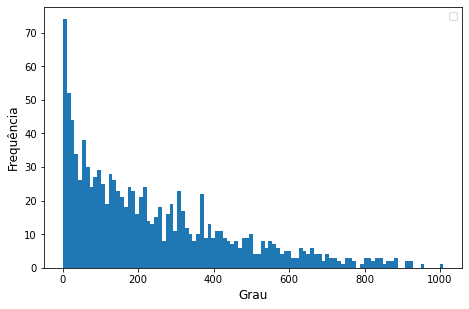
\includegraphics[scale=0.6]{images/base-de-dados-29-degree-distribution-cnae.png}
    \label{fig:metricas-redes:base-de-dados-29-degree-distribution-cnae}
    \fdadospesquisa
\end{figure}

A rede também apresenta uma transitividade significativa que reflete a conectividade da rede e uma tendência leve à desassortatividade de grau. A assortatividade de seção não indicou nenhuma tendência, indicando que não existe preferência dos vértices de se conectarem ou não à vértices da mesma seção.

As Tabelas~\ref{tab:metricas-redes:grafo-por-cnae-especificas1} e \ref{tab:metricas-redes:grafo-por-cnae-especificas2} apresentam a distribuição das outras métricas estudadas. Novamente, foram usadas as formulações utilizando arestas ponderadas para o estudo.

\begin{table}[htb]
\centering
\caption{Métricas do grafo de transações entre CNAEs segmentadas por CNAE (Parte 1)}
\label{tab:metricas-redes:grafo-por-cnae-especificas1}
\begin{tabular}{l|rrrrr}
\toprule
Métrica & Grau & \shortstack{Coeficiente\\de agrupamento} & Excentricidade & \shortstack{Caminho\\mínimo médio} & \shortstack{Caminho mínimo\\médio ponderado} \\
\midrule
Média         &  241.1 &   $1.471e^{-05}$ & 2.917 & 1.8160 & $1.140e^{-05}$ \\
Desvio Padrão &  213.7 &   $1.946e^{-05}$ & 0.309 & 0.2289 & $6.641e^{-05}$ \\
Mínimo        &    1   &                0 &     2 & 1.1030 & $5.708e^{-06}$ \\
25º percentil &   66   &   $4.441e^{-06}$ &     3 & 1.6800 & $5.722e^{-06}$ \\
50º percentil &  183   &   $9.605e^{-06}$ &     3 & 1.8470 & $5.776e^{-06}$ \\
75º percentil &  365   &   $1.790e^{-05}$ &     3 & 1.9640 & $6.351e^{-06}$ \\
Máximo        & 1009   &           0.0003 &     4 & 2.7970 &         0.0019 \\
\bottomrule
\end{tabular}
\fdadospesquisa
\end{table}

\begin{table}[htb]
\centering
\caption{Métricas do grafo de transações entre CNAEs segmentadas por CNAE (Parte 2)}
\label{tab:metricas-redes:grafo-por-cnae-especificas2}
\begin{tabular}{l|rrrrr}
\toprule
Métrica & \shortstack{Centralidade\\de informação} & \shortstack{Centralidade\\de autovalor} & \shortstack{Centralidade de\\intermediação} & \shortstack{Centralidade\\de proximidade} & PageRank \\
\midrule
Média         & 225.9    &         0.0020 &         0.0007 & 0.5598 & 0.0008 \\
Desvio Padrão &  47.49   &         0.0298 &         0.0019 & 0.0769 & 0.0021 \\
Mínimo        &   0.4702 & $3.198e^{-12}$ &              0 & 0.3572 & 0.0001 \\
25º percentil & 235.5    & $3.452e^{-07}$ & $3.047e^{-06}$ & 0.5086 & 0.0001 \\
50º percentil & 245.4    & $5.856e^{-06}$ & $5.415e^{-05}$ & 0.5409 & 0.0002 \\
75º percentil & 246.3    & $7.721e^{-05}$ &         0.0005 & 0.5947 & 0.0007 \\
Máximo        & 246.4     &         0.8161 &         0.0287 & 0.9057 & 0.0316 \\
\bottomrule
\end{tabular}
\fdadospesquisa
\end{table}

Analisando a distribuição do coeficiente de agrupamento, é possível verificar que existe uma certa variância que indicam a presença de alguns vértices com agrupamento local significativo, embora a magnitude da métrica seja bastante influenciada pelo fato de usar a formulação para arestas ponderadas. Por outro lado, a excentricidade dos vértices apresenta pouca variância o que reflete uma rede curta, de baixo diâmetro e raio, da mesma forma que a distribuição do caminho mínimo médio partindo dos vértices também possui uma variância limitada e fortemente correlacionada ao grau.

As métricas de centralidade de informação, de proximidade e de proximidade são novamente influenciadas pelo volume transacionado por cada CNAE e sofrem certo efeito também do baixo comprimento da rede, apresentando uma variância também baixa. Já a centralidade de autovalor e o pagerank apresentam variância significativa possivelmente refletindo o valor total transacionado pelos vértices e não sendo tão influenciados pela topologia da rede.

\subsection{Conclusões}
\label{section:metricas-redes:conclusoes}

Assim, fica claro a partir da caracterização das redes com dados de 2019 que são redes com topologias não tão complexas e que possuem uma forte correlação com os valores transacionados por cada entidade. Apesar disso, este estudo pode adicionar informações importantes sobre a topologia dessas redes que serão usadas no estudo do impacto da pandemia do ponto de vista topológico e podem ser usados para a detecção ou decisão de entidades que tiveram impacto da pandemia.

\section{Alterações topológicas}
\label{section:alteracoes-topologicas}

Nesta seção, vamos analisar mudanças que ocorreram na estrutura das redes para o período da pandemia em comparação com a topologia vista na caracterização anterior.

\subsection{Redes UF-UF}
\label{section:alteracoes-topologicas:uf}

\begin{table}[htb]
\centering
\caption{Variação percentual das métricas de redes mês a mês para o grafo de UFs (Parte 1)}
\label{tab:metricas-redes-pandemia:grafo-mensal-por-uf1}
\begin{tabular}{l|rrrr}
\toprule
Mês & Densidade & Transitividade & Grau médio & \shortstack{Grau médio\\ponderado} \\
\midrule
01/2019 & - & - & - & - \\
02/2019 & +0.54\% & +0.55\% & +0.54\% &  +9.88\% \\
03/2019 & +0.00\% & +0.17\% & +0.00\% & +25.54\% \\
04/2019 & +0.54\% & +0.57\% & +0.54\% & +23.86\% \\
05/2019 & +0.81\% & +0.81\% & +0.81\% & +36.91\% \\
06/2019 & +0.27\% & +0.32\% & +0.27\% & +23.88\% \\
07/2019 & +0.54\% & +0.57\% & +0.54\% & +28.36\% \\
08/2019 & +0.54\% & +0.57\% & +0.54\% & +35.37\% \\
09/2019 & +0.27\% & +0.36\% & +0.27\% & +32.62\% \\
10/2019 & +0.81\% & +0.82\% & +0.81\% & +42.89\% \\
11/2019 & +0.27\% & +0.34\% & +0.27\% & +43.93\% \\
12/2019 & +0.27\% & +0.36\% & +0.27\% & +29.66\% \\
01/2020 & +0.81\% & +0.83\% & +0.81\% & +28.84\% \\
02/2020 & +0.27\% & +0.44\% & +0.27\% & +32.22\% \\
03/2020 & +0.54\% & +0.59\% & +0.54\% & +36.09\% \\
04/2020 & -0.27\% & -0.07\% & -0.27\% &  -7.91\% \\
05/2020 & -0.27\% & -0.18\% & -0.27\% & +12.47\% \\
06/2020 & +0.00\% & +0.11\% & +0.00\% & +34.61\% \\
07/2020 & +0.54\% & +0.57\% & +0.54\% & +62.51\% \\
08/2020 & +0.54\% & +0.59\% & +0.54\% & +55.16\% \\
09/2020 & +1.08\% & +1.09\% & +1.08\% & +60.32\% \\
10/2020 & +0.00\% & +0.17\% & +0.00\% & +61.19\% \\
\bottomrule
\end{tabular}
\fdadospesquisa
\end{table}

Primeiramente, vamos analisar alterações topológicas na estrutura das redes UF-UF no período que compreende janeiro de 2019 e outubro de 2020. Para esta análise, os dados foram dividido mês a mês e um grafo foi criado para cada mês do período estudado. Cada vértice destes grafos representa uma UF e cada aresta representa o valor total transacionado entre duas UFs naquele mês. Usamos novamente a modelagem de grafo cíclico ponderado, sendo que cada aresta possui novamente um atributo indicando a distância entre os vértices igual ao inverso do valor transacionado. Cada vértice possui também um atributo indicando a região a qual pertence aquela UF, usado em uma das métricas de assortatividade.

A Tabelas~\ref{tab:metricas-redes-pandemia:grafo-mensal-por-uf1} e \ref{tab:metricas-redes-pandemia:grafo-mensal-por-uf2} mostram a evolução de algumas métricas gerais das redes UF-UF para cada mês do período analisado. Cada linha da tabela representa o valor da métrica analisada em relação ao mês de janeiro de 2019, mostrando assim a evolução percentual em relação a esse mês-base.

\begin{table}[htb]
\centering
\caption{Variação das métricas de redes mês a mês para o grafo de UFs (Parte 2)}
\label{tab:metricas-redes-pandemia:grafo-mensal-por-uf2}
\begin{tabular}{l|rrrr}
\toprule
Mês & \shortstack{Assortatividade\\de grau} & \shortstack{Assortatividade\\de região} & \shortstack{Caminho mínimo\\médio} & \shortstack{Caminho mínimo\\médio ponderado} \\
\midrule
01/2019 & - & - & - & - \\
02/2019 & -15.60\% & -50.13\% & -0.55\% &  -8.47\% \\
03/2019 &  +0.05\% &  -0.00\% & +0.00\% & -25.12\% \\
04/2019 &  +7.91\% & -15.39\% & -0.55\% & -22.23\% \\
05/2019 & -31.31\% & -85.53\% & -0.83\% & -25.07\% \\
06/2019 & +21.99\% & +13.35\% & -0.27\% &  +2.44\% \\
07/2019 & -17.07\% & -57.33\% & -0.55\% &  -1.69\% \\
08/2019 &  +7.91\% & -57.33\% & -0.55\% & -11.02\% \\
09/2019 &  +4.73\% & -28.82\% & -0.27\% &  -2.55\% \\
10/2019 &  -6.87\% & -43.83\% & -0.83\% & -11.15\% \\
11/2019 &  +8.56\% & +13.35\% & -0.27\% & -14.48\% \\
12/2019 &  +4.73\% & -70.86\% & -0.27\% &  +2.50\% \\
01/2020 & -25.43\% & -43.83\% & -0.83\% &  +1.69\% \\
02/2020 & -18.97\% & -28.82\% & -0.27\% &  -5.58\% \\
03/2020 &  -7.22\% & -15.39\% & -0.55\% &  -4.69\% \\
04/2020 &  +1.98\% & -13.38\% & +0.27\% & +36.70\% \\
05/2020 & +37.79\% & +29.14\% & +0.27\% &  +2.72\% \\
06/2020 & +19.66\% & -42.28\% & +0.00\% & -15.66\% \\
07/2020 &  +7.91\% & -15.39\% & -0.55\% & -32.97\% \\
08/2020 &  -7.22\% & -15.39\% & -0.55\% & -35.56\% \\
09/2020 & -16.88\% & -71.96\% & -1.11\% & -37.64\% \\
10/2020 &  +0.05\% & -42.28\% &  0.00\% & -30.06\% \\
\bottomrule
\end{tabular}
\fdadospesquisa
\end{table}

A partir desses dados, é possível ver que as oscilações mês a mês nas métricas são pequenas, muitas vezes menor que 1\%. Quando analisamos as densidade, transitividade, e grau médio, podemos ver que nos meses de abril e maio de 2020 há uma queda pequena mas consistente em todas essas métricas. Isso mostra uma pequena perda de de conectividade geral da rede, que se recupera e retoma os níveis anteriores a partir de agosto de 2020. Analisando o grau médio ponderado, uma métrica que envolve valores transacionados, podemos ver que a variância nos meses anteriores à crise é maior, em patamares de dezenas de pontos percentuais, e da mesma forma o impacto da crise nos meses de abril e maio é mais significativo, chegando a ser 7\% menor que o mês-base.

Analisando a assortatividade de grau e de região, podemos notar também uma variância mais significativa a partir dos dados nos meses que precedem a pandemia. Não há uma tendência clara em nenhuma dessas métricas, sendo que elas oscilam positivamente e negativamente no decorrer do tempo e não podemos deduzir que a variação para os meses de maior impacto da pandemia tem relação com a crise. No mês de maio, há um aumento pontual de ambas assortatividades, mas logo retornando às variações e aos patamares anteriores nos meses seguintes.

Ao observar o caminho mínimo médio verificamos uma variância pequena nos meses que precedem a pandemia, tendendo a encurtar os caminhos mínimos em relação ao mês-base, e nos meses do segundo trimestre de 2020 há um aumento tímido mas consistente desta métrica, voltando aos patamares anteriores após esse período. Utilizando a análise de caminhos mínimos ponderados observamos uma variação maior dos dados, novamente com tendência de diminuição da métrica nos meses que precedem a pandemia em relação ao mês base, sendo que nos meses de abril e maio a métrica tem um aumento consideravelmente consistente e depois alcança um patamar de alta diminuição dos caminhos mínimos em relação ao mês-base.

\begin{table}[htb]
\centering
\caption{Variação das métricas de rede a cada trimestre para o grafo de UFs (Parte 1)}
\label{tab:metricas-redes-pandemia:grafo-trimestral-por-uf1}
\begin{tabular}{l|rrrr}
\toprule
Mês & Densidade & Transitividade & Grau médio & \shortstack{Grau médio\\ponderado} \\
\midrule
2020/1 & - & - & - & - \\
2020/2 & -0.80\% & -0.78\% & -0.80\% & -14.60\% \\
2020/3 & +0.27\% & +0.22\% & +0.27\% & +20.35\% \\
\bottomrule
\end{tabular}
\fdadospesquisa
\end{table}

\begin{table}[htb]
\centering
\caption{Variação das métricas de rede a cada trimestre para o grafo de UFs (Parte 2)}
\label{tab:metricas-redes-pandemia:grafo-trimestral-por-uf2}
\begin{tabular}{l|rrrr}
\toprule
Mês & \shortstack{Assortatividade\\de grau} & \shortstack{Assortatividade\\de região} & \shortstack{Caminho mínimo\\médio} & \shortstack{Caminho mínimo\\médio ponderado} \\
\midrule
2020/1 & - & - & - & - \\
2020/2 & +77.29\% &  +1.84\% & +0.85\% &  +6.63\% \\
2020/3 & -34.35\% & -83.36\% & -0.28\% & -33.74\% \\
\bottomrule
\end{tabular}
\fdadospesquisa
\end{table}

É possível traçar uma relação entre a diminuição da conectividade e o aumento dos caminhos mínimos, uma vez que tais métricas são naturalmente inversamente proporcionais: quanto mais conectado é uma rede, menor são os caminhos mínimos necessários para percorrê-la. Isso não significa necessariamente uma relação causal, uma vez que a perda de conectividade da rede foi aparentemente bastante pequena, apesar de consistente.

Por fim, analisamos as Tabelas~\ref{tab:metricas-redes-pandemia:grafo-trimestral-por-uf1} e \ref{tab:metricas-redes-pandemia:grafo-trimestral-por-uf2} que repetem a mesma análise, mas agora com grafos utilizando dados trimestrais ao invés de mensais. São mantidas as mesmas regras de formação dos grafos conforme a descrição anterior. A análise agora passa a ser em relação ao primeiro trimestre de 2020, que tomamos como trimestre-base.

Novamente, é possível observar perda de conectividade na rede em pequenos mas consistentes percentuais, afetando as métricas densidade, transitividade, grau médio, e grau médio ponderado. Essa conectividade é aparentemente recuperada no trimestre posterior. Por outro lado, as redes apresentam um ganho significativo de assortatividade de grau, indicando preferência dos vértices de se conectar a vértices semelhantes. A assortatividade de região e as métricas de caminhos mínimos médios apresentaram tímido aumento percentual. Essas outras métricas tiveram queda no trimestre seguinte, em sentido contrário ao apresentado.

% \begin{table}[htb]
% \centering
% \caption{Diferença entre as métricas de rede para UFs afetadas e não afetadas}
% \label{tab:metricas-redes-pandemia:diferenca-afetadas-por-uf}
% \begin{tabular}{l|rrrrrrr}
% \toprule
% Métrica & Média & \shortstack{Desvio\\padrão} & Mínimo & P25 & Mediana & P75 & Máximo \\
% \midrule
% Grau médio                     & -1.85\% &   +2.51\% &  -0.26\% & -3.70\% &  +0.00\% &  +0.00\% &    +0.00\% \\ \hline
% \shortstack[l]{Coeficiente de\\agrupamento}     &  +0.33\% &   +4.71\% &   +2.79\% & -2.34\% & -0.83\% &  6.67\% &  -14.51\% \\ \hline
% Excentricidade                 & -4.17\% & -20.41\% &   +0.00\% &  +0.00\% &  +0.00\% &  +0.00\% & -100.00\% \\ \hline
% \shortstack[l]{Caminho mínimo\\médio}           &  +1.85\% &   +2.46\% &   +0.00\% &  +0.00\% &  +0.00\% &  +3.70\% &   -0.28\% \\ \hline
% \shortstack[l]{Caminho mínimo\\médio ponderado} & -6.58\% &   +0.14\% &  -2.01\% & -7.36\% & -0.36\% & -1.03\% &  -37.83\% \\ \hline
% \shortstack[l]{Centralidade de\\proximidade}    & -1.71\% &   +2.28\% &   +0.25\% & -3.45\% &  +0.00\% &  +0.00\% &    +0.00\% \\ \hline
% \shortstack[l]{Centralidade de\\informação}     & -1.07\% &  -1.71\% &   +9.93\% & -1.09\% &  +0.16\% &  +0.10\% &   -8.60\% \\ \hline
% \shortstack[l]{Centralidade de\\autovalor}      & -3.84\% &  -1.85\% &  +23.00\% & -0.99\% & -1.58\% & -4.25\% &  -20.99\% \\ \hline
% \shortstack[l]{Centralidade de\\intermediação}  &  - &     - & 206.06\% &  +0.00\% &  +0.00\% &  +0.00\% &    - \\ \hline
% PageRank                       & -0.63\% &   +0.02\% &   +4.37\% & -1.23\% & -1.61\% & -1.01\% &   -5.26\% \\
% \bottomrule
% \end{tabular}
% \fdadospesquisa
% \end{table}

\subsection{Redes Seção-Seção}
\label{section:alteracoes-topologicas:secao}

\begin{table}[htb]
\centering
\caption{Variação percentual das métricas de redes mês a mês para o grafo de seções (Parte 1)}
\label{tab:metricas-redes-pandemia:grafo-mensal-por-secao1}
\begin{tabular}{l|rrrr}
\toprule
Mês & Densidade & Transitividade & Grau médio & \shortstack{Grau médio\\ponderado} \\
\midrule
01/2019 &  - &  - &  - &  - \\
02/2019 & -0.57\% & -0.55\% & -0.57\% &  +9.89\%\\
03/2019 & +0.57\% & +0.31\% & +0.57\% & +25.54\%\\
04/2019 & -1.15\% & -1.20\% & -1.15\% & +23.86\%\\
05/2019 & +1.15\% & +0.15\% & +1.15\% & +36.92\%\\
06/2019 & -1.72\% & -1.33\% & -1.72\% & +23.89\%\\
07/2019 & -0.57\% & -1.00\% & -0.57\% & +28.37\%\\
08/2019 & -0.57\% & -0.63\% & -0.57\% & +35.37\%\\
09/2019 & +0.00\% & +0.18\% & +0.00\% & +32.63\%\\
10/2019 & -0.57\% & +0.13\% & -0.57\% & +42.89\%\\
11/2019 & -1.72\% & -1.25\% & -1.72\% & +43.94\%\\
12/2019 & +1.15\% & +0.85\% & +1.15\% & +29.66\%\\
01/2020 & +2.30\% & +1.87\% & +2.30\% & +28.85\%\\
02/2020 & +1.15\% & +0.46\% & +1.15\% & +32.22\%\\
03/2020 & +1.72\% & +0.98\% & +1.72\% & +36.10\%\\
04/2020 & -0.57\% & -0.38\% & -0.57\% &  -7.92\%\\
05/2020 & -0.57\% & -0.47\% & -0.57\% & +12.47\%\\
06/2020 & -1.72\% & -0.72\% & -1.72\% & +34.62\%\\
07/2020 & -1.72\% & -1.97\% & -1.72\% & +62.52\%\\
08/2020 & +0.00\% & -0.15\% & +0.00\% & +55.16\%\\
09/2020 & +1.72\% & +1.24\% & +1.72\% & +60.33\%\\
10/2020 & +0.00\% & -0.60\% & +0.00\% & +61.20\%\\
\bottomrule
\end{tabular}
\fdadospesquisa
\end{table}

A seguir, serão analisadas alterações topológicas na estrutura das redes Seção-Seção no período que compreende janeiro de 2019 e outubro de 2020. Nesta análise, os dados foram mais uma vez dividido mês a mês e um grafo foi criado para cada mês do período estudado. Cada vértice destes grafos representa uma seção e cada aresta representa o valor total transacionado entre duas seções naquele mês. Usamos novamente a modelagem de grafo cíclico ponderado, sendo que cada aresta possui novamente um atributo indicando a distância entre os vértices igual ao inverso do valor transacionado.

As Tabelas~\ref{tab:metricas-redes-pandemia:grafo-mensal-por-secao1} e \ref{tab:metricas-redes-pandemia:grafo-mensal-por-secao2} apresentam a evolução das métricas das redes Seção-Seção para cada mês. Cada linha mostra portanto a variação do valor das métricas do grafo montado para aquele mês em relação ao mês de janeiro de 2019, usado novamente como mês-base.

Assim como nas redes UF-UF, temos aqui uma baixa variação nos dados das métricas de densidade, transitividade, e grau médio, sendo que a magnitude da variação dessas métricas é menor que 2.5\%, o que dificulta afirmações mais assertivas. Para essas três métricas, não existe uma tendência clara de crescimento ou redução de cada métrica no decorrer do tempo, sendo que comparando os meses imediatamente anteriores à crise com os meses mais críticos (abril e maio de 2020), há uma aparente queda de densidade e transitividade indicando uma leve redução na conectividade da rede, que apresenta evolução nos meses seguintes. Quando observamos o grau médio ponderado, uma métrica influenciada pelo volume mensal de transações, podemos então ver que nos meses mais críticos da crise o grau médio diminuiu, indicando um menor fluxo de transações entre os vértices das redes.

Ao analisar a assortatividade de grau podemos ver uma variação nessas métricas sem tendência clara de crescimento ou redução para todo o período analisado. A métrica caminho mínimo médio também apresenta uma variação sem tendência clara e com baixa magnitude, com uma leve alta nos meses mais críticos da crise em relação aos meses imediatamente anteriores, mas não sendo o suficiente para indicar uma tendência. Quando analisamos o grau médio ponderado por outro lado, métrica influenciada pelo volume de transações, podemos verificar que nos meses de abril e maio de 2020 há uma variação significativa que indica aumento desta métrica em relação aos meses imediatamente anteriores e posteriores.

As Tabelas~\ref{tab:metricas-redes-pandemia:grafo-trimestral-por-secao1} e \ref{tab:metricas-redes-pandemia:grafo-trimestral-por-secao2} mostram a mesma análise mas do ponto de vista trimestral em relação ao primeiro trimestre de 2020, tomado como trimestre-base.

\begin{table}[htb]
\centering
\caption{Variação das métricas de redes mês a mês para o grafo de seções (Parte 2)}
\label{tab:metricas-redes-pandemia:grafo-mensal-por-secao2}
\begin{tabular}{l|rrrr}
\toprule
Mês & \shortstack{Assortatividade\\de grau} & \shortstack{Caminho mínimo\\médio} & \shortstack{Caminho mínimo\\médio ponderado} \\
\midrule
01/2019 &  - &  - &  - \\
02/2019 &  +2.76\% & +0.45\% & +29.22\% \\
03/2019 &  -9.42\% & -0.45\% & -11.35\% \\
04/2019 &  +4.86\% & +0.90\% &  +2.19\% \\
05/2019 &  +1.47\% & -0.45\% &  +3.75\% \\
06/2019 & +16.41\% & +0.90\% &  +5.20\% \\
07/2019 &  +1.48\% & +0.45\% & -15.91\% \\
08/2019 &  +6.16\% & +0.45\% & -13.54\% \\
09/2019 &  -5.13\% & -0.45\% & -10.76\% \\
10/2019 &  -1.58\% & +0.00\% & -15.12\% \\
11/2019 &  10.43\% & +0.90\% & -38.71\% \\
12/2019 &  -3.53\% & -0.90\% & -41.20\% \\
01/2020 & -14.48\% & -1.80\% & -25.39\% \\
02/2020 &  -1.24\% & -0.45\% & -36.64\% \\
03/2020 &  -7.40\% & -0.90\% & +22.58\% \\
04/2020 &  -4.91\% & +0.45\% & +28.02\% \\
05/2020 &  -8.57\% & +0.45\% & +114.33\% \\
06/2020 &  -3.99\% & +1.35\% & +72.81\% \\
07/2020 &  -4.68\% & +1.80\% & +65.47\% \\
08/2020 & -11.69\% & +0.45\% & +60.28\% \\
09/2020 & -10.17\% & -0.90\% & +56.97\% \\
10/2020 &  -6.61\% & +0.45\% & -33.58\% \\
\bottomrule
\end{tabular}
\fdadospesquisa
\end{table}

Ao observarmos agora de forma agregada os dados trimestrais de 2020, podemos ver pela densidade, transitividade, e grau médio que há uma leve redução na conectividade da rede nos trimestres após o começo da pandemia em relação ao trimestre-base. Quando incluímos o grau médio ponderado, vemos que há uma queda significativa no segundo trimestre em relação ao trimestre-base e que há recuperação no trimestre seguinte.

A seguir, verificamos uma tendência de alta da assortatividade de grau durante o trimestre mais crítico da crise, retornando ao patamar anterior no trimestre seguinte. E ao analisar o caminho mínimo médio podemos ver que não há variação significativa em relação ao trimestre-base, mas quando fazemos a análise da métrica ponderada é possível verificar um aumento considerável no distância entre os vértices da rede.

\begin{table}[htb]
\centering
\caption{Variação das métricas de rede a cada trimestre para o grafo de seções (Parte 1)}
\label{tab:metricas-redes-pandemia:grafo-trimestral-por-secao1}
\begin{tabular}{l|rrrr}
\toprule
Mês & Densidade & Transitividade & Grau médio & \shortstack{Grau médio\\ponderado} \\
\midrule
2020/1 & - & - & - & - \\
2020/2 & -1.66\% & -0.92\% & -1.66\% & -14.60\% \\
2020/3 & -1.10\% & -0.59\% & -1.10\% & +20.35\% \\
\bottomrule
\end{tabular}
\fdadospesquisa
\end{table}

\begin{table}[htb]
\centering
\caption{Variação das métricas de rede a cada trimestre para o grafo de seções (Parte 2)}
\label{tab:metricas-redes-pandemia:grafo-trimestral-por-secao2}
\begin{tabular}{l|rrrr}
\toprule
Mês & \shortstack{Assortatividade\\de grau} & \shortstack{Caminho mínimo\\médio} & \shortstack{Caminho mínimo\\médio ponderado} \\
\midrule
2020/1 & - & - & - & - \\
2020/2 & +11.16\% & +0.93\% & +122.98\% \\
2020/3 &  -2.87\% & +0.93\% & +100.19\% \\
\bottomrule
\end{tabular}
\fdadospesquisa
\end{table}

% \begin{table}[htb]
% \centering
% \caption{Diferença entre as métricas de rede para seções afetadas e não afetadas}
% \label{tab:metricas-redes-pandemia:diferenca-afetadas-por-secao}
% \begin{tabular}{l|rrrrrrr}
% \toprule
% Métrica & Média & \shortstack{Desvio\\padrão} & Mínimo & P25 & Mediana & P75 & Máximo \\
% \midrule
% Grau médio                     &  +0.02\% & -0.04\% & +0.11\% & +0.05\% &  +0.00\% &  +0.00\% & -0.05\% \\ \hline
% \shortstack[l]{Coeficiente de\\agrupamento}     &  +0.16\% & -0.01\% & +0.38\% & +0.15\% &  +0.11\% &  +0.14\% &  +0.07\% \\ \hline
% Excentricidade                 &  +0.00\% &  +0.00\% & +0.00\% & +0.00\% &  +0.00\% &  +0.00\% &  +0.00\% \\ \hline
% \shortstack[l]{Caminho mínimo\\médio}           & -0.01\% & -0.03\% & +0.05\% & +0.00\% &  +0.00\% & -0.04\% & -0.05\% \\ \hline
% \shortstack[l]{Caminho mínimo\\médio ponderado} &  +0.00\% & -0.00\% & +0.00\% & +0.00\% & -0.00\% & -0.00\% & -0.00\% \\ \hline
% \shortstack[l]{Centralidade de\\proximidade}    &  +0.01\% & -0.03\% & +0.05\% & +0.04\% &  +0.00\% &  +0.00\% & -0.05\% \\ \hline
% \shortstack[l]{Centralidade de\\informação}     &  +0.00\% & -0.00\% & +0.00\% & +0.00\% &  +0.00\% & -0.00\% & -0.00\% \\ \hline
% \shortstack[l]{Centralidade de\\autovalor}      &  +0.32\% & -0.00\% & +0.56\% & +0.39\% &  +0.20\% &  +0.25\% &  +0.28\% \\ \hline
% \shortstack[l]{Centralidade de\\intermediação}  &  +0.43\% &  +0.12\% & +0.76\% & +0.34\% &  +0.00\% &  +0.46\% &  +0.00\% \\ \hline
% PageRank                       &  +0.07\% & -0.04\% & +0.17\% & +0.07\% &  +0.08\% &  +0.11\% & -0.21\% \\
% \bottomrule
% \end{tabular}
% \fdadospesquisa
% \end{table}

\subsection{Redes CNAE-CNAE}
\label{section:alteracoes-topologicas:cnae}

Por fim, serão apresentadas as alterações topológicas na estrutura das redes CNAE-CNAE no período que compreende janeiro de 2019 e outubro de 2020.

\begin{table}[htb]
\centering
\caption{Variação percentual das métricas de redes mês a mês para o grafo de CNAEs (Parte 1)}
\label{tab:metricas-redes-pandemia:grafo-mensal-por-cnae1}
\begin{tabular}{l|rrrr}
\toprule
Mês & Densidade & Transitividade & Grau médio & \shortstack{Grau médio\\ponderado} \\
\midrule
01/2019 & - & - & - & - \\
02/2019 &  +4.35\% &  +1.75\% &  +4.45\% &  +9.79\% \\
03/2019 &  +5.96\% &  +2.29\% &  +6.15\% & +25.32\% \\
04/2019 &  +9.60\% &  +3.67\% &  +9.70\% & +23.75\% \\
05/2019 & +11.46\% &  +4.22\% & +11.66\% & +36.67\% \\
06/2019 &  +7.55\% &  +2.71\% &  +7.55\% & +23.89\% \\
07/2019 & +12.16\% &  +4.16\% & +12.06\% & +28.48\% \\
08/2019 & +12.70\% &  +4.64\% & +12.80\% & +35.25\% \\
09/2019 & +11.38\% &  +4.45\% & +11.48\% & +32.51\% \\
10/2019 & +13.87\% &  +5.36\% & +14.27\% & +42.38\% \\
11/2019 & +12.57\% &  +4.84\% & +12.67\% & +43.81\% \\
12/2019 &  +6.15\% &  +2.35\% &  +6.62\% & +29.09\% \\
01/2020 &  +9.87\% &  +3.64\% & +10.27\% & +28.39\% \\
02/2020 &  +8.58\% &  +3.01\% &  +8.87\% & +31.87\% \\
03/2020 &  +9.29\% &  +3.80\% &  +9.68\% & +35.62\% \\
04/2020 &  -2.40\% &  -0.24\% &  -2.40\% &  -7.92\% \\
05/2020 &  +1.98\% &  +1.67\% &  +2.07\% & +12.37\% \\
06/2020 &  +7.94\% &  +3.99\% &  +8.13\% & +34.38\% \\
07/2020 & +11.86\% &  +5.21\% & +12.46\% & +61.65\% \\
08/2020 & +10.99\% &  +4.48\% & +10.89\% & +55.30\% \\
09/2020 &  +9.68\% &  +4.69\% & +10.26\% & +59.47\% \\
10/2020 &  +7.63\% &  +3.96\% &  +8.02\% & +60.62\% \\
\bottomrule
\end{tabular}
\fdadospesquisa
\end{table}

Da mesma forma, os dados foram dividido mês a mês e um grafo foi criado para cada mês do período estudado. Cada vértice destes grafos representa um CNAE e cada aresta representa o valor total transacionado entre dois CNAEs naquele mês. Usamos novamente a modelagem de grafo cíclico ponderado, sendo que cada aresta possui novamente um atributo indicando a distância entre os vértices igual ao inverso do valor transacionado. Cada vértice possui também um atributo indicando a seção a que pertence aquele CNAE para uso na métrica de assortatividade.

As Tabelas~\ref{tab:metricas-redes-pandemia:grafo-mensal-por-cnae1} e \ref{tab:metricas-redes-pandemia:grafo-mensal-por-cnae2} apresentam as métricas desta análise, apresentando a variação percentual de cada métrica para cada mês em relação ao mês-base de janeiro de 2019.

\begin{table}[htb]
\centering
\caption{Variação das métricas de redes mês a mês para o grafo de CNAEs (Parte 2)}
\label{tab:metricas-redes-pandemia:grafo-mensal-por-cnae2}
\begin{tabular}{l|rrrr}
\toprule
Mês & \shortstack{Assortatividade\\de grau} & \shortstack{Assortatividade\\de seção} & \shortstack{Caminho mínimo\\médio} & \shortstack{Caminho mínimo\\médio ponderado} \\
\midrule
01/2019 & - & - & - & - \\
02/2019 &  +0.38\% &  -6.76\% & -0.72\% &  -9.37\% \\
03/2019 &  +1.52\% & -22.04\% & -0.93\% & +35.22\% \\
04/2019 &  +1.80\% &  -8.60\% & -1.49\% & +33.50\% \\
05/2019 &  +2.69\% & -23.49\% & -1.83\% & -13.22\% \\
06/2019 &  +1.02\% & -24.50\% & -1.15\% & -15.84\% \\
07/2019 &  +1.76\% &  +4.38\% & -1.77\% & -17.73\% \\
08/2019 &  +1.77\% & -16.28\% & -1.64\% &  +3.81\% \\
09/2019 &  +0.86\% &  +3.95\% & -1.65\% & -29.89\% \\
10/2019 &  +1.55\% &  -4.69\% & -1.83\% & -35.86\% \\
11/2019 &  +1.02\% &  -8.01\% & -1.83\% & -36.74\% \\
12/2019 &  +0.52\% & -10.46\% & -1.08\% & -30.56\% \\
01/2020 &  +2.06\% &  -6.52\% & -1.50\% & -28.02\% \\
02/2020 &  +1.27\% &  +9.35\% & -1.30\% & -23.95\% \\
03/2020 &  +1.61\% &  +1.73\% & -1.40\% & -23.14\% \\
04/2020 &  -0.02\% &  +8.10\% & +0.58\% &  -8.54\% \\
05/2020 &  +1.14\% & +16.10\% & -0.27\% &  +9.73\% \\
06/2020 &  +2.35\% &  +0.88\% & -1.13\% & +16.51\% \\
07/2020 &  +3.60\% & +15.25\% & -1.66\% &  +1.86\% \\
08/2020 &  +1.83\% & +12.58\% & -1.57\% & -26.79\% \\
09/2020 &  +2.24\% & +16.47\% & -1.21\% &  +5.56\% \\
10/2020 &  +1.30\% &  -4.01\% & -0.98\% & -17.64\% \\
\bottomrule
\end{tabular}
\fdadospesquisa
\end{table}

Mais uma vez, podemos verificar a redução da conectividade das redes através da densidade, da transitividade e do grau médio da rede em relação ao mês-base, com as três métricas apresentando redução em relação aos meses imediatamente anteriores ao início da crise e se recuperando nos meses posteriores aos meses mais críticos. Essa métricas agora apresentam uma variação de magnitude significativa, sendo mais importante que nas redes analisadas anteriormente. Se considerarmos o grau médio ponderado essa diferença se torna ainda mais significativa, também com tendência de redução durante os meses mais críticos e posterior recuperação.

Analisando a assortatividade de grau das redes, é possível ver que existe pouca variação em relação ao mês-base, e que no mês de abril de 2020 há uma variação diferente para leve disassortatividade, voltando para os patamares anteriores nos meses seguintes. Já quando observamos a assortatividade de seção, vemos uma variação de magnitude mais significativa, e que apresenta tendência positiva nos meses da pandemia que se mantém até setembro de 2020. Essa tendência de aumento na assortatividade de seção é interessante pois indicaria que na rede de CNAEs as seções tem alguma preferência de se conectar com seções semelhantes.

Por fim, analisando o caminho mínimo médio, é possível verificar certa estabilidade no período analisado em relação ao mês-base, com exceção dos meses de abril de maio de 2020 quando aparentemente há um aumento da distância entre os vértices das redes. Quando incluímos ponderação pelo valor transacionado na análise, essa diferença se torna ainda mais evidente, com uma alta que impacta também meses posteriores aos meses mais críticos.

\begin{table}[htb]
\centering
\caption{Variação das métricas de rede a cada trimestre para o grafo de CNAEs (Parte 1)}
\label{tab:metricas-redes-pandemia:grafo-trimestral-por-cnae1}
\begin{tabular}{l|rrrr}
\toprule
Mês & Densidade & Transitividade & Grau médio & \shortstack{Grau médio\\ponderado} \\
\midrule
2020/1 & - & - & - & - \\
2020/2 & -4.91\% & -1.09\% & -4.91\% & -14.60\% \\
2020/3 & +0.82\% & +0.98\% & +0.91\% & +20.25\% \\
\bottomrule
\end{tabular}
\fdadospesquisa
\end{table}

\begin{table}[htb]
\centering
\caption{Variação das métricas de rede a cada trimestre para o grafo de CNAEs (Parte 2)}
\label{tab:metricas-redes-pandemia:grafo-trimestral-por-cnae2}
\begin{tabular}{l|rrrr}
\toprule
Mês & \shortstack{Assortatividade\\de grau} & \shortstack{Assortatividade\\de seção} & \shortstack{Caminho mínimo\\médio} & \shortstack{Caminho mínimo\\médio ponderado} \\
\midrule
2020/1 & - & - & - & - \\
2020/2 & -0.21\% & +8.07\% & +0.98\% & +71.35\% \\
2020/3 & +0.66\% & +3.81\% & +0.05\% & +26.02\% \\
\bottomrule
\end{tabular}
\fdadospesquisa
\end{table}

As Tabelas~\ref{tab:metricas-redes-pandemia:grafo-trimestral-por-cnae1} e \ref{tab:metricas-redes-pandemia:grafo-trimestral-por-cnae2} complementam a análise anterior fazendo novamente a análise agora agregando os dados em trimestres e mostrando a variação em relação ao primeiro trimestre de 2020, o trimestre-base.

Novamente, podemos verificar a perda de conectividade da rede no trimestre mais crítico, o segundo de 2020, com uma redução na densidade, transitividade, e grau médio da rede, apresentando uma retomada no trimestre seguinte. Incluindo o grau médio ponderado, novamente essa variação se mostra mais evidente.

Por fim, analisando a variação das métricas de assortatividade, a assortatividade de grau apresenta leve redução no trimestre mais crítico seguida de leve retomada no trimestre seguinte. A assortatividade de seção apresenta alta no trimestre mais crítico e regularização no trimestre seguinte. A distância entre os vértices medida através do caminho mínimo médio apresenta leve tendência de alta nos trimestres da pandemia e se acentuam quando usamos a análise da métrica ponderada.

% \begin{table}[htb]
% \centering
% \caption{Diferença entre as métricas de rede para CNAEs afetadas e não afetadas}
% \label{tab:metricas-redes-pandemia:diferenca-afetadas-por-cnae}
% \begin{tabular}{l|rrrrrrr}
% \toprule
% Métrica & Média & \shortstack{Desvio\\padrão} & Mínimo & P25 & Mediana & P75 & Máximo \\
% \midrule
% Grau médio                     &  0.02\% & -0.04\% & 0.11\% & 0.05\% &  0.00\% &  0.00\% & -0.05\% \\ \hline
% \shortstack[l]{Coeficiente de\\agrupamento}     &  0.16\% & -0.01\% & 0.38\% & 0.15\% &  0.11\% &  0.14\% &  0.07\% \\ \hline
% Excentricidade                 &  0.00\% &  0.00\% & 0.00\% & 0.00\% &  0.00\% &  0.00\% &  0.00\% \\ \hline
% \shortstack[l]{Caminho mínimo\\médio}           & -0.01\% & -0.03\% & 0.05\% & 0.00\% &  0.00\% & -0.04\% & -0.05\% \\ \hline
% \shortstack[l]{Caminho mínimo\\médio ponderado} &  0.00\% & -0.00\% & 0.00\% & 0.00\% & -0.00\% & -0.00\% & -0.00\% \\ \hline
% \shortstack[l]{Centralidade de\\proximidade}    &  0.01\% & -0.03\% & 0.05\% & 0.04\% &  0.00\% &  0.00\% & -0.05\% \\ \hline
% \shortstack[l]{Centralidade de\\informação}     &  0.00\% & -0.00\% & 0.00\% & 0.00\% &  0.00\% & -0.00\% & -0.00\% \\ \hline
% \shortstack[l]{Centralidade de\\autovalor}      &  0.32\% & -0.00\% & 0.56\% & 0.39\% &  0.20\% &  0.25\% &  0.28\% \\ \hline
% \shortstack[l]{Centralidade de\\intermediação}  &  0.43\% &  0.12\% & 0.76\% & 0.34\% &  0.00\% &  0.46\% &  0.00\% \\ \hline
% PageRank                       &  0.07\% & -0.04\% & 0.17\% & 0.07\% &  0.08\% &  0.11\% & -0.21\% \\
% \bottomrule
% \end{tabular}
% \fdadospesquisa
% \end{table}

\subsection{Conclusões}
\label{section:alteracoes-topologicas:conclusoes}

Nesta seção, fizemos uma descrição da oscilação de diversas métricas de redes através e uma modelagem temporal, comparando com as redes se comportam através do tempo e eventuais tendências.

Para o estudo das redes de topologia mais simples, UF-UF e Seção-Seção, a variação das métricas apresentou uma variação de baixa magnitude, muitas vezes menor que 1\%, mas puderam apresentar algumas tendências consistentes mesmo assim. Pudemos ver que mesmo nessas redes há uma perda de conectividade das redes, principalmente nos meses e trimestres mais críticos, evidenciada quando levamos em consideração as formulações que levam em conta os valores transacionados.

As redes CNAE-CNAE que tem uma topologia mais complexa apresentaram a mesma tendência mas de forma mais significativa, sendo que pudemos observar uma magnitude maior nas variações de cada métricas, refletindo da mesma a perda de conectividade da rede.

A perda de conectividade é um sintoma citado nos trabalhos descritos na seção~\ref{introducao:crise-economica}, que analisam dados de áreas significativamente diferentes, como o transporte aéreo global. Assim como o trabalho citado sobre a correlação do impacto da pandemia no mercado de ações apontava para um aumento do caminho mínimo médio, uma tendência também encontrada neste trabalho.

\section{Detecção de impacto econômico}
\label{section:deteccao-impacto}

Nesta seção, nas últimas seções pudemos verificar como a base de dados analisada se comportou durante a pandemia, sob diferentes perspectivas. Agora vamos apresentar os métodos tentados para a detecção e classificação de impacto econômico, visando tentar identificar de forma automatizada entidades afetadas pela crise sob diferentes modelagens. Todos os conjuntos de dados a seguir foram normalizados utilizando norma euclideana, ou norma L2.

\subsection{Dados de UFs}
\label{section:deteccao-impacto:uf}

Para esta análise, criamos uma matriz foram reunidos os dados descritos na seção~\ref{section:metricas-redes:uf}, as métricas de caracterização da rede UF-UF, com algumas métricas relacionadas ao volume transacionado por cada UF: volume total, quantidade de transações, e valor médio de cada transação. Assim, foi criada uma matriz onde cada linha representa uma UF e cada coluna o valor de uma das métricas de redes ou de transações, totalizando onze variáveis.

Também foi uma criada uma segunda tabela com o impacto mensal e total para cada UF, conforme descrito na seção~\ref{section:impacto:cenario-regional}. O objetivo aqui é observar o comportamento de classificadores ao tentar decidir a partir dos dados das métricas obtidas se é possível classificar uma UF como impactada ou não.

\begin{figure}[htb]
	\centering
    \caption{Percentual de variância explicada de cada componente principal para dados de UFs}
    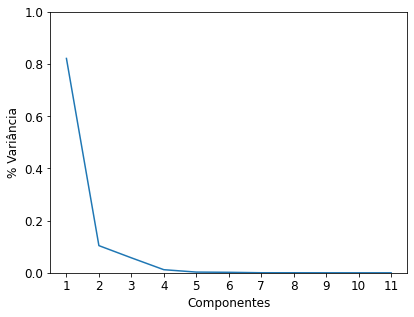
\includegraphics[scale=0.7]{images/base-de-dados-24.1-pca-components-monthly-uf.png}
    \label{fig:resultados:base-de-dados-24-pca-monthly-uf}
    \fdadospesquisa
\end{figure}

Foi feita uma análise de componentes principais a partir dos dados. A Figura~\ref{fig:resultados:base-de-dados-24-pca-monthly-uf} ilustra o percentual da variância explicada pelo conjunto de dados explicada por cada componente principal. As duas primeiras componentes principais concentram a maior parte da variância explicada pelo conjunto de dados.

\begin{table}[htb]
\centering
\caption{Direção de cada métrica em relação a cada uma das duas componentes principais}
\label{tab:resultados:direcao-components-uf}
\begin{tabular}{l|rrrr}
\toprule
Componente & 1 & 2 \\
\midrule
Valor total                    &  0.4746 &  0.1108 \\
Quantidade de transações       &  0.4708 &  0.1544 \\
Valor médio por transação      & -0.0077 & -0.3831 \\
Grau                           &  0.0009 & -0.0101 \\
Coeficiente de agrupamento     &  0.3311 & -0.2535 \\
Excentricidade                 & -0.0226 &  0.2543 \\
Caminho mínimo médio           & -0.0010 &  0.0108 \\
Caminho mínimo médio ponderado & -0.1081 &  0.7227 \\
Centralidade de informação     &  0.0976 & -0.3850 \\
Centralidade de autovalores    &  0.4783 &  0.1268 \\
PageRank                       &  0.4392 &  0.0377 \\
\bottomrule
\end{tabular}
\fdadospesquisa
\end{table}

Na Tabela~\ref{tab:resultados:direcao-components-uf} são descritas as direções de cada variável em relação à cada uma das duas componentes principais. Para a primeira componente se destacam a magnitude do valor total e da quantidade de transações, além da centralidade de autovalores e de informação, enquanto para a segunda componente se destacam o valor médio por transação e novamente a centralidade de informação. As variáveis com maior magnitude terão maior impacto decisivo nos classificadores que usaremos posteriormente.

As Figuras~\ref{fig:resultados:base-de-dados-24.2-pca-2d-monthly-uf} e \ref{fig:resultados:base-de-dados-25.2-pca-2d-total-uf} ilustram a projeção dos dados em relação às duas componentes principais para dar uma noção do espalhamento dos dados, em relação respectivamente ao impacto mensal e impacto total.

\begin{figure}[htb] 
    \centering 
    \caption{Visualização dos dados de UFs projetados sobre as duas componentes principais}
    \label{fig:resultados:pca-uf}
    \begin{subfigure}[b]{0.45\textwidth}
        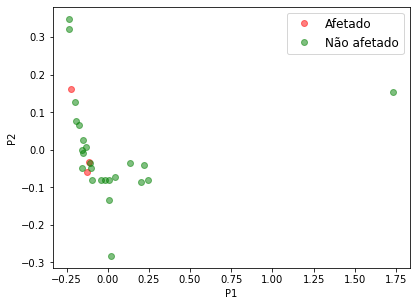
\includegraphics[scale=0.45]{images/base-de-dados-24.2-pca-2d-monthly-uf.png}
        \caption{Impacto mensal}
        \label{fig:resultados:base-de-dados-24.2-pca-2d-monthly-uf}
    \end{subfigure} ~ \quad
    \begin{subfigure}[b]{0.45\textwidth}
        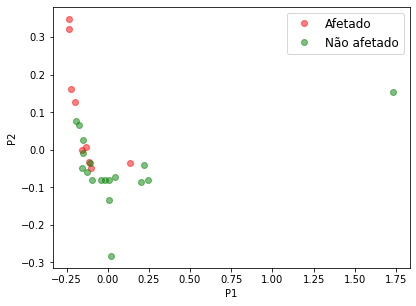
\includegraphics[scale=0.45]{images/base-de-dados-25.2-pca-2d-total-uf.png}
        \caption{Impacto total}
        \label{fig:resultados:base-de-dados-25.2-pca-2d-total-uf}
    \end{subfigure}
    \fdadospesquisa
\end{figure}

O conjunto de dados possui algum espalhamento nos dados, e parece ter algumas UFs um pouco mais distantes do restante. Porém, não existem regiões onde é clara a distinção de afetados e não afetados tanto para o impacto mensal quanto total. No caso do impacto total, existem UFs afetadas que parecem ocupar uma região próxima onde essas poderiam ser separadas linearmente, enquanto outras permanecem em uma região pouco divisível. Também é importante notar que ambos conjuntos de dados são desbalanceados, o que é um desafio para classificadores.

Ao aplicarmos classificadores sobre os dados foram obtidos os resultados ilustrados nas Figuras~\ref{fig:base-de-dados-24.1-confusion-matrix-monthly-uf}, \ref{fig:base-de-dados-24.1-confusion-matrix-total-uf1} e \ref{fig:base-de-dados-24.1-confusion-matrix-total-uf2}. A primeira se refere aos dados de impacto mensal e as seguintes ao impacto total, conforme descrito anteriormente. Para validação da técnica, foi utilizado o método \textit{leave-one-out}. 

Para a tentativa de classificação dos dados de UFs para impacto mensal, três classificadores tiveram o mesmo resultado: Random Forest, Regressão Logística, e SVC, onde todas as UFs foram classificadas como positivos. Já utilizando o classificador KNN, o resultado foi semelhante mas uma das UFs que deveria ser classificada como positivo foi agora classificada como negativo. Apesar de uma alta acurácia, o resultado não é interessante uma vez que temos uma grande quantidade de falsos positivos para todos os métodos, faltando generalização.

\begin{figure}[htb] 
    \centering 
    \caption{Matrizes de confusão para classificadores aplicados sobre dados de UFs para impacto mensal}
    \label{fig:base-de-dados-24.1-confusion-matrix-monthly-uf}
    \begin{subfigure}[b]{0.45\textwidth}
        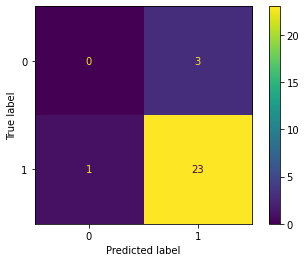
\includegraphics[scale=0.75]{images/base-de-dados-24.3-confusion-matrix-knn-monthly-uf.png}
        \caption{KNN}
        \label{fig:resultados:base-de-dados-24.3-confusion-matrix-knn-monthly-uf}
    \end{subfigure} ~ \quad
    \begin{subfigure}[b]{0.45\textwidth}
        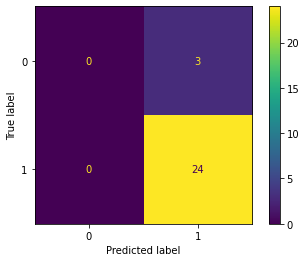
\includegraphics[scale=0.75]{images/base-de-dados-24.1-confusion-matrix-randomforest-monthly-uf.png}
        \caption{Random Forest, Regressão Logística, e SVC}
        \label{fig:resultados:base-de-dados-24.1-confusion-matrix-randomforest-monthly-uf}
    \end{subfigure}
    \fdadospesquisa
\end{figure}

Para os dados de impacto total, o resultado foi um pouco mais positivo. As maiores acurácias foram apresentadas pelos classificadores Regressão Logística e SVC, com cerca de 70\%, seguido de KNN com 66\% e Regressão Logística com 59\%. Evidentemente, a acurácia para este conjunto de dados desbalanceado esconde um grande problema dessa classificação, que é conseguir uma boa especificidade para este conjuntos de dados. Todos os classificadores tiveram problemas com a quantidade de falsos positivos e falsos negativos. Nenhum dos classificadores portanto conseguiu efetivamente alcançar uma generalização aceitável.

\begin{figure}[htb] 
    \centering 
    \caption{Matrizes de confusão para classificadores aplicados sobre dados de UFs para impacto total (Parte 1)}
    \label{fig:base-de-dados-24.1-confusion-matrix-total-uf1}
    \begin{subfigure}[b]{0.45\textwidth}
        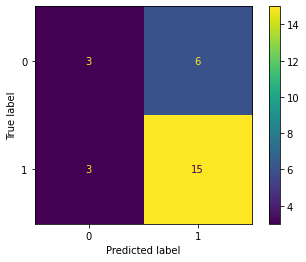
\includegraphics[scale=0.75]{images/base-de-dados-24.3-confusion-matrix-knn-total-uf.png}
        \caption{KNN}
        \label{fig:resultados:base-de-dados-24.3-confusion-matrix-knn-total-uf}
    \end{subfigure} ~ \quad
    \begin{subfigure}[b]{0.45\textwidth}
        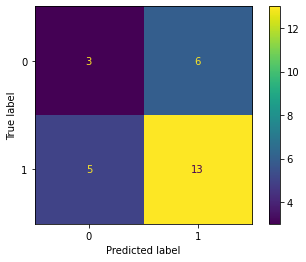
\includegraphics[scale=0.75]{images/base-de-dados-24.1-confusion-matrix-randomforest-total-uf.png}
        \caption{Random Forest}
        \label{fig:resultados:base-de-dados-24.1-confusion-matrix-randomforest-total-uf}
    \end{subfigure}
\end{figure}
\begin{figure}[htb] 
    \centering 
    \caption{Matrizes de confusão para classificadores aplicados sobre dados de UFs para impacto total (Parte 2)}
    \label{fig:base-de-dados-24.1-confusion-matrix-total-uf2}
    \begin{subfigure}[b]{0.45\textwidth}
        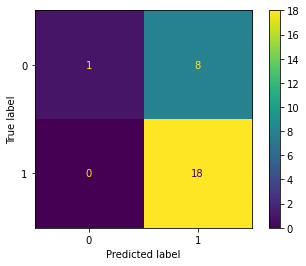
\includegraphics[scale=0.75]{images/base-de-dados-24.1-confusion-matrix-logisticregression-total-uf.png}
        \caption{Regressão Logística}
        \label{fig:resultados:base-de-dados-24.3-confusion-matrix-logisticregression-total-uf}
    \end{subfigure} ~ \quad
    \begin{subfigure}[b]{0.45\textwidth}
        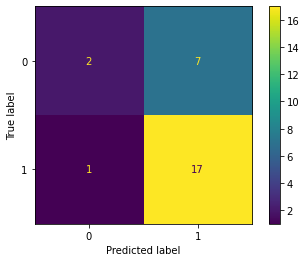
\includegraphics[scale=0.75]{images/base-de-dados-24.2-confusion-matrix-svc-total-uf.png}
        \caption{SVC}
        \label{fig:resultados:base-de-dados-24.1-confusion-matrix-svc-total-uf}
    \end{subfigure}
    \fdadospesquisa
\end{figure}

% \begin{table}[htb]
% \centering
% \caption{Métricas de classificação do impacto mensal de cada método para os dados de UFs}
% \label{tab:resultados:classification-report-monthly-uf}
% \begin{tabular}{l|r|rrrr}
% \toprule
% Método & Métrica & Negativos & Positivos & Média & \shortstack{Média\\ponderada} \\
% \midrule
% \multirow{4}{*}{KNN} & Precisão & 0.0000 &  0.8750 &  0.4375 &  0.7778 \\
%  & Recall   & 0.0000 &  0.8750 &  0.4375 &  0.7778 \\
%  & F1-Score & 0.0000 &  0.8750 &  0.4375 &  0.7778 \\
%  & Suporte  & 3.0000 & 24.0000 & 27.0000 & 27.0000 \\ \hline
% \multirow{4}{*}{Random forest} & Precisão & 0.0000 &  0.8889 &  0.4444 &  0.7901 \\
%  & Recall   & 0.0000 &  1.0000 &  0.5000 &  0.8889 \\
%  & F1-Score & 0.0000 &  0.9412 &  0.4706 &  0.8366 \\
%  & Suporte  & 3.0000 & 24.0000 & 27.0000 & 27.0000 \\ \hline
% \multirow{4}{*}{Regressão Logística} & Precisão & 0.0000 &  0.8889 &  0.4444 &  0.7901 \\
%  & Recall   & 0.0000 &  1.0000 &  0.5000 &  0.8889 \\
%  & F1-Score & 0.0000 &  0.9412 &  0.4706 &  0.8366 \\
%  & Suporte  & 3.0000 & 24.0000 & 27.0000 & 27.0000 \\ \hline
% \multirow{4}{*}{SVC} & Precisão & 0.0000 &  0.8889 &  0.4444 &  0.7901 \\
%  & Recall   & 0.0000 &  1.0000 &  0.5000 &  0.8889 \\
%  & F1-Score & 0.0000 &  0.9412 &  0.4706 &  0.8366 \\
%  & Suporte  & 3.0000 & 24.0000 & 27.0000 & 27.0000 \\
% \bottomrule
% \end{tabular}
% \fdadospesquisa
% \end{table}

\subsection{Dados de Seções}
\label{section:deteccao-impacto:secao}

Repetimos então a análise, construindo uma matriz agora usando os dados de seções, com os dados descritos na seção~\ref{section:metricas-redes:secao} junto das métricas de volume total, quantidade de transações, e valor médio de transações.

\begin{figure}[htb]
	\centering
    \caption{Percentual de variância explicada de cada componente principal para dados de seções}
    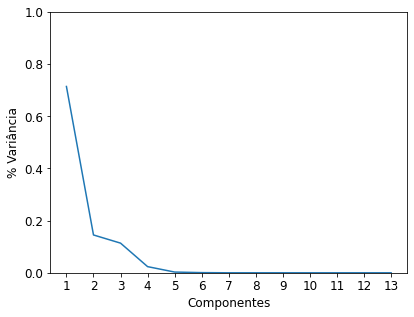
\includegraphics[scale=0.7]{images/base-de-dados-26.1-pca-components-monthly-secao.png}
    \label{fig:resultados:base-de-dados-24-pca-monthly-secao}
    \fdadospesquisa
\end{figure}

A matriz resultante possui uma linha para cada seção analisada e uma coluna para cada métrica, totalizando treze variáveis. Utilizamos também os dados de impacto mensal e total por seção descritos na seção~\ref{section:impacto:cenario-economico}.

\begin{table}[htb]
\centering
\caption{Direção de cada métrica em relação a cada uma das duas componentes principais para os dados de seções}
\label{tab:resultados:direcao-components-secao}
\begin{tabular}{l|rrrr}
\toprule
Componente & 1 & 2 \\
\midrule
Valor total                    &  0.4238 &  0.0153 \\
Quantidade de transações       &  0.3972 &  0.0648 \\
Valor médio por transação      & -0.0133 & -0.5534 \\
Grau                           &  0.0243 & -0.1738 \\
Coeficiente de agrupamento     &  0.3633 & -0.0632 \\
Excentricidade                 & -0.0702 & -0.0082 \\
Caminho mínimo médio           & -0.0195 &  0.1362 \\
Caminho mínimo médio ponderado & -0.0504 &  0.7709 \\
Centralidade de proximidade    &  0.0171 & -0.0829 \\
Centralidade de informação     &  0.0120 & -0.1816 \\
Centralidade de autovalores    &  0.4237 &  0.0396 \\
PageRank                       &  0.4121 &  0.0084 \\
Centralidade de intermediação  &  0.4151 &  0.0285 \\
\bottomrule
\end{tabular}
\fdadospesquisa
\end{table}

Assim como anteriormente, foi aplicada a análise das componentes principais dessa matriz. A Figura~\ref{fig:resultados:base-de-dados-24-pca-monthly-secao} mostra o percentual da variância total explicada pelo conjunto de dados para cada componente. Novamente, as duas primeiras componentes explicam a maior parte da variância do conjunto de dados.

\begin{figure}[htb] 
    \centering 
    \caption{Visualização dos dados de seções projetados sobre as duas componentes principais}
    \label{fig:resultados:pca-secao}
    \begin{subfigure}[b]{0.45\textwidth}
        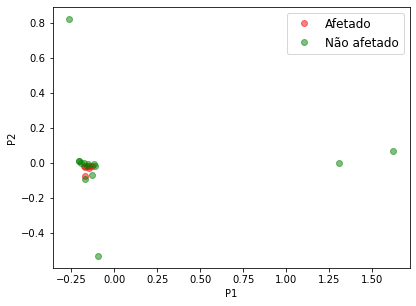
\includegraphics[scale=0.45]{images/base-de-dados-26.2-pca-2d-monthly-secao.png}
        \caption{Impacto mensal}
        \label{fig:resultados:base-de-dados-26.2-pca-2d-monthly-secao}
    \end{subfigure} ~ \quad
    \begin{subfigure}[b]{0.45\textwidth}
        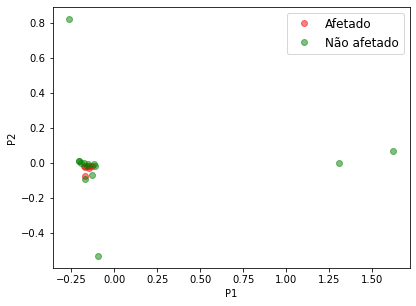
\includegraphics[scale=0.45]{images/base-de-dados-27.2-pca-2d-total-secao.png}
        \caption{Impacto total}
        \label{fig:resultados:base-de-dados-27.2-pca-2d-total-secao}
    \end{subfigure}
    \fdadospesquisa
\end{figure}

A seguir, na Tabela~\ref{tab:resultados:direcao-components-secao}, é descrita a direção de cara variável em relação às duas principais componentes. O valor total novamente tem uma participação importante, mas as métricas de centralidade de autovalores, \textit{pagerank}, e centralidade de intermediação apresentam também magnitude significativa em relação à primeira componente, enquanto as maiores magnitudes para a segundo componentes pertencem às váriáveis valor médio por transação e caminho mínimo médio ponderado.

A Figura~\ref{fig:resultados:pca-secao} apresenta o espalhamento dos dados projetos sobre as duas componentes principais representando o impacto mensal e total. É possível ver que os dados são pouco espalhados e se concentram em uma região principal do espaço de variáveis, além de possuir quatro seções distantes com um aparente comportamento de \textit{outliers}. Novamente, os dados são bastante desbalanceados.

\begin{figure}[htb] 
    \centering 
    \caption{Matrizes de confusão para classificadores aplicados sobre dados de seções para impacto mensal}
    \label{fig:base-de-dados-24.1-confusion-matrix-monthly-secao}
    \begin{subfigure}[b]{0.45\textwidth}
        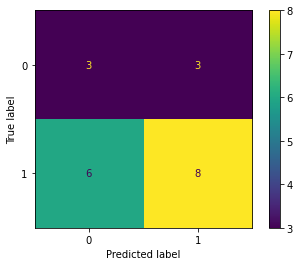
\includegraphics[scale=0.75]{images/base-de-dados-24.3-confusion-matrix-knn-monthly-secao.png}
        \caption{KNN}
        \label{fig:resultados:base-de-dados-24.3-confusion-matrix-knn-monthly-secao}
    \end{subfigure} ~ \quad
    \begin{subfigure}[b]{0.45\textwidth}
        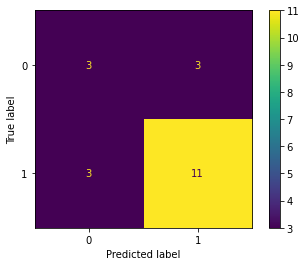
\includegraphics[scale=0.75]{images/base-de-dados-24.1-confusion-matrix-randomforest-monthly-secao.png}
        \caption{Random Forest}
        \label{fig:resultados:base-de-dados-24.1-confusion-matrix-randomforest-monthly-secao}
    \end{subfigure} \\
    \begin{subfigure}[b]{0.45\textwidth}
        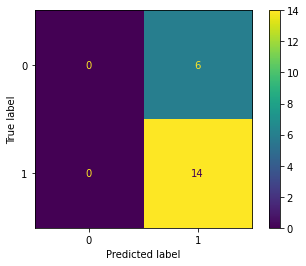
\includegraphics[scale=0.75]{images/base-de-dados-24.1-confusion-matrix-logisticregression-monthly-secao.png}
        \caption{Regressão Logística}
        \label{fig:resultados:base-de-dados-24.3-confusion-matrix-logisticregression-monthly-secao}
    \end{subfigure} ~ \quad
    \begin{subfigure}[b]{0.45\textwidth}
        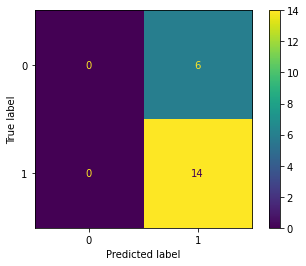
\includegraphics[scale=0.75]{images/base-de-dados-24.2-confusion-matrix-svc-monthly-secao.png}
        \caption{SVC}
        \label{fig:resultados:base-de-dados-24.1-confusion-matrix-svc-monthly-secao}
    \end{subfigure}
    \fdadospesquisa
\end{figure}

\begin{figure}[htb] 
    \centering 
    \caption{Matrizes de confusão para classificadores aplicados sobre dados de seções para impacto total}
    \label{fig:base-de-dados-24.1-confusion-matrix-total-secao}
    \begin{subfigure}[b]{0.45\textwidth}
        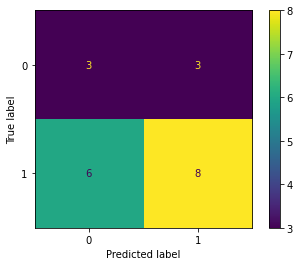
\includegraphics[scale=0.75]{images/base-de-dados-24.3-confusion-matrix-knn-total-secao.png}
        \caption{KNN}
        \label{fig:resultados:base-de-dados-24.3-confusion-matrix-knn-total-secao}
    \end{subfigure} ~ \quad
    \begin{subfigure}[b]{0.45\textwidth}
        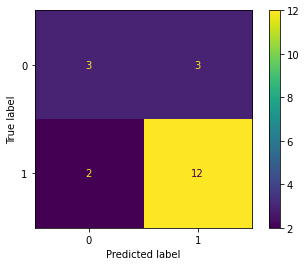
\includegraphics[scale=0.75]{images/base-de-dados-24.1-confusion-matrix-randomforest-total-secao.png}
        \caption{Random Forest}
        \label{fig:resultados:base-de-dados-24.1-confusion-matrix-randomforest-total-secao}
    \end{subfigure} \\
    \begin{subfigure}[b]{0.45\textwidth}
        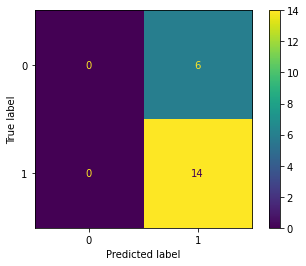
\includegraphics[scale=0.75]{images/base-de-dados-24.1-confusion-matrix-logisticregression-total-secao.png}
        \caption{Regressão Logística}
        \label{fig:resultados:base-de-dados-24.3-confusion-matrix-logisticregression-total-secao}
    \end{subfigure} ~ \quad
    \begin{subfigure}[b]{0.45\textwidth}
        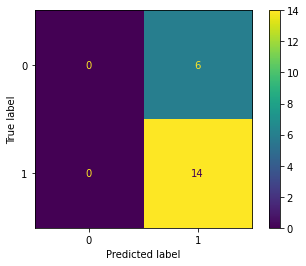
\includegraphics[scale=0.75]{images/base-de-dados-24.2-confusion-matrix-svc-total-secao.png}
        \caption{SVC}
        \label{fig:resultados:base-de-dados-24.1-confusion-matrix-svc-total-secao}
    \end{subfigure}
    \fdadospesquisa
\end{figure}

Foram aplicados também classificadores sobre os dados, que são ilustrados nas Figuras~\ref{fig:base-de-dados-24.1-confusion-matrix-monthly-secao} e \ref{fig:base-de-dados-24.1-confusion-matrix-total-secao}, referentes ao impacto mensal e total respectivamente. Para a validação foi novamente utilizada a técnica \textit{leave-one-out}.

Novamente, os classificadores não foram capazes de apresentar boa generalização sobre os dados, sendo que dois deles classificaram todas as seções como afetadas pela crise. O classificador KNN apresentou baixa precisão, com uma alta taxa de falsos positivos. E o classificador Random Forest apresentou um resultado razoável, com uma acurácia de 70\%, precisão de 78\% e especificidade de 50\%.

\subsection{Dados de CNAEs}
\label{section:deteccao-impacto:cnae}

Por fim, aplicamos a mesma técnica anterior sobre os dados de CNAEs.

\begin{figure}[htb]
	\centering
    \caption{Percentual de variância explicada de cada componente principal para dados de CNAEs}
    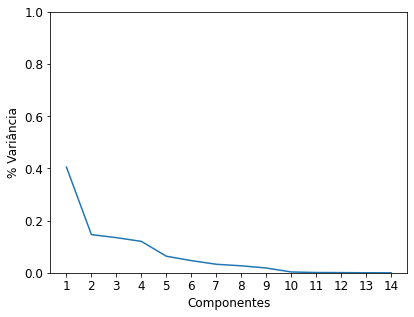
\includegraphics[scale=0.7]{images/base-de-dados-28.1-pca-components-monthly-cnae.png}
    \label{fig:resultados:base-de-dados-24-pca-monthly-cnae}
    \fdadospesquisa
\end{figure}

Montamos uma matriz novamente agregando os dados de volume total transacionado, quantidade de transações, valor médio de transações, seção do CNAE (discretizada), e as métricas de redes da seção~\ref{section:metricas-redes:cnae}, totalizando catorze variáveis.

\begin{table}[htb]
\centering
\caption{Direção de cada métrica em relação a cada uma das duas componentes principais para os dados de CNAEs}
\label{tab:resultados:direcao-components-cnae}
\begin{tabular}{l|rrrr}
\toprule
Componente & 1 & 2 & 3 & 4 \\
\midrule
Seção                          &  0.5035 & -0.0108 &  0.0966 &  0.0441 \\
Valor total                    &  0.4563 &  0.3150 & -0.0079 & -0.1132 \\
Quantidade de transações       &  0.0612 & -0.4170 &  0.6541 &  0.1840 \\
Valor médio por transação      &  0.1895 & -0.2848 & -0.3259 &  0.0631 \\
Grau                           &  0.1765 & -0.3230 &  0.3309 &  0.1040 \\
Coeficiente de agrupamento     & -0.0217 &  0.0357 &  0.0442 & -0.0124 \\
Excentricidade                 & -0.0328 &  0.0529 &  0.0559 & -0.0012 \\
Caminho mínimo médio           & -0.0295 &  0.3470 & -0.0146 &  0.9292 \\
Caminho mínimo médio ponderado &  0.0388 & -0.0607 & -0.0697 &  0.0092 \\
Centralidade de proximidade    &  0.0207 & -0.0689 & -0.0039 & -0.0521 \\
Centralidade de informação     &  0.4090 &  0.4709 &  0.1726 & -0.1805 \\
Centralidade de autovalores    &  0.4696 & -0.1466 &  0.0038 &  0.0944 \\
PageRank                       &  0.2737 & -0.3887 & -0.5499 &  0.1673 \\
Centralidade de intermediação  & -0.0225 &  0.1185 & -0.0681 &  0.0283 \\
\bottomrule
\end{tabular}
\fdadospesquisa
\end{table}

A Figura~\ref{fig:resultados:base-de-dados-24-pca-monthly-cnae} apresenta o percentual da variância explicada pelo conjunto de dados para cada componente principal dessa matriz. Ao contrário dos conjuntos anteriores, há maior distribuição da variância explicada por entre as componentes. São necessárias agora quatro componentes principais para totalizar 80.6\% da variância total do conjunto de dados.

A Tabela~\ref{tab:resultados:direcao-components-cnae} mostra a direção de cada variável em relação a cada uma das quatro componentes principais. Algumas métricas já citadas nas análises anteriores novamente se sobressaem: valor total, quantidade de transações, centralidade de informação, centralidade de autovalores, \textit{pagerank}. A variável seção, adicionada para melhorar o espalhamento dos dados, também tem participação importante principalmente na primeira componente principal.

A Figura~\ref{fig:resultados:base-de-dados-24-pca-monthly-cnae} mostra o espalhamento dos dados projetados sobre as duas componentes principais em relação ao impacto mensal e total. É possível novamente ver que não há um espalhamento significativo, com exceção de alguns \textit{outliers}, e as duas classes se sobrepõem uma a outra sem regiões bem definidas. O conjunto considerando impacto mensal é bastante desbalanceado, enquanto o conjunto que considera impacto total é menos desbalanceado.

\begin{figure}[htb] 
    \centering 
    \caption{Visualização dos dados de CNAEs projetados sobre as duas componentes principais}
    \label{fig:resultados:pca-cnae}
    \begin{subfigure}[b]{0.45\textwidth}
        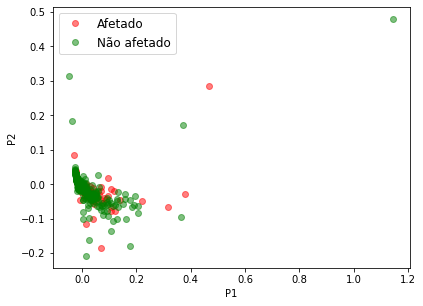
\includegraphics[scale=0.45]{images/base-de-dados-28.2-pca-2d-monthly-cnae.png}
        \caption{Impacto mensal}
        \label{fig:resultados:base-de-dados-24.2-pca-2d-monthly-cnae}
    \end{subfigure} ~ \quad
    \begin{subfigure}[b]{0.45\textwidth}
        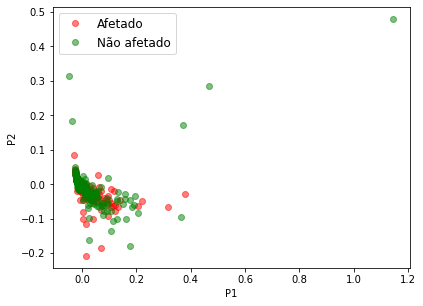
\includegraphics[scale=0.45]{images/base-de-dados-28.2-pca-2d-total-cnae.png}
        \caption{Impacto total}
        \label{fig:resultados:base-de-dados-25.2-pca-2d-total-cnae}
    \end{subfigure}
    \fdadospesquisa
\end{figure}

Mais uma vez aplicamos classificadores sobre os dados para identificação do impacto mensal e total. Desta vez, dado o tamanho do dataset utilizados a técnica k-fold estratificado para validarmos os dados obtidos através dos classificadores. As Figuras~\ref{fig:resultados:classification-monthly-cnae} e \ref{fig:resultados:classification-total-cnae} mostram os resultados obtidos, através das matrizes de confusão e curva ROC.

Para o conjunto de dados de impacto mensal, novamente os classificadores falharam em identificar verdadeiros negativos. O classificador que melhor conseguiu generalizar os dados foi novamente Random Forest, com uma precisão de 95\% mas uma especificidade de apenas 12\%. Também para o conjunto de dados de impacto total, significativamente mais balanceado, os resultados apresentaram pouca generalização. Todos os métodos apresentaram uma alta taxa de falsos positivos e negativos.

\begin{figure}[htb] 
    \centering 
    \caption{Resultado das tentativas de classificação para cada método aplicado sobre dados de CNAEs para impacto mensal}
    \label{fig:resultados:classification-monthly-cnae} 
    \begin{subfigure}[b]{0.45\textwidth}
        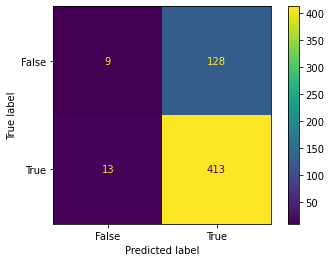
\includegraphics[scale=0.55]{images/base-de-dados-28.3.5-confusion-matrix-knn-monthly-cnae.png}
        \caption{Matriz de confusão para KNN}
        \label{fig:resultados:base-de-dados-28.3.5-confusion-matrix-knn-monthly-cnae}
    \end{subfigure} ~ \quad
    \begin{subfigure}[b]{0.45\textwidth}
        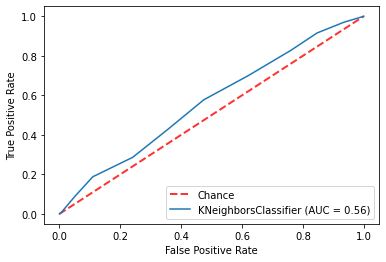
\includegraphics[scale=0.55]{images/base-de-dados-28.3.6-roc-curve-knn-monthly-cnae.png}
        \caption{Curva ROC para KNN}
        \label{fig:resultados:base-de-dados-28.3.6-roc-curve-knn-monthly-cnae}
    \end{subfigure} ~ \\
    \begin{subfigure}[b]{0.45\textwidth}
        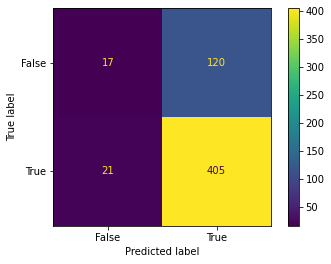
\includegraphics[scale=0.55]{images/base-de-dados-28.3.1-confusion-matrix-randomforest-monthly-cnae.png}
        \caption{Matriz de confusão para Random Forest}
        \label{fig:resultadosbase-de-dados-28.3.1-confusion-matrix-randomforest-monthly-cnae}
    \end{subfigure} ~ \quad
    \begin{subfigure}[b]{0.45\textwidth}
        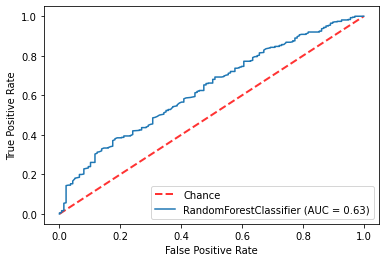
\includegraphics[scale=0.55]{images/base-de-dados-28.3.2-roc-curve-randomforest-monthly-cnae.png}
        \caption{Curva ROC para Random Forest}
        \label{fig:resultados:base-de-dados-28.3.2-roc-curve-randomforest-monthly-cnae}
    \end{subfigure} ~ \\
    \begin{subfigure}[b]{0.45\textwidth}
        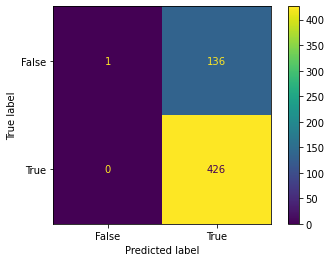
\includegraphics[scale=0.55]{images/base-de-dados-28.3.7-confusion-matrix-logregression-monthly-cnae.png}
        \caption{Matriz de confusão para Regressão logística}
        \label{fig:resultados:base-de-dados-28.3.7-confusion-matrix-logregression-monthly-cnae}
    \end{subfigure} ~ \quad
    \begin{subfigure}[b]{0.45\textwidth}
        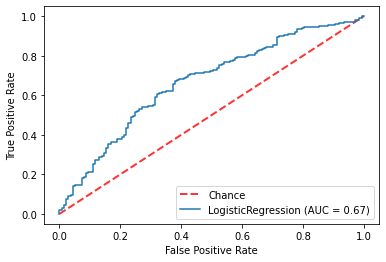
\includegraphics[scale=0.55]{images/base-de-dados-28.3.8-roc-curve-logregression-monthly-cnae.png}
        \caption{Curva ROC para Regressão Logística}
        \label{fig:resultados:base-de-dados-28.3.8-roc-curve-logregression-monthly-cnae}
    \end{subfigure} ~ \\
        \begin{subfigure}[b]{0.45\textwidth}
        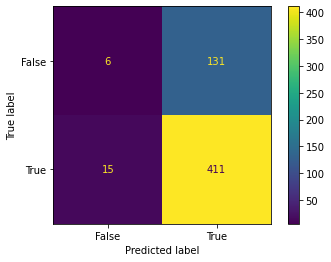
\includegraphics[scale=0.55]{images/base-de-dados-28.3.3-confusion-matrix-svc-monthly-cnae.png}
        \caption{Matriz de confusão para SVC}
        \label{fig:resultados:base-de-dados-28.3.3-confusion-matrix-svc-monthly-cnae}
    \end{subfigure} ~ \quad
    \begin{subfigure}[b]{0.45\textwidth}
        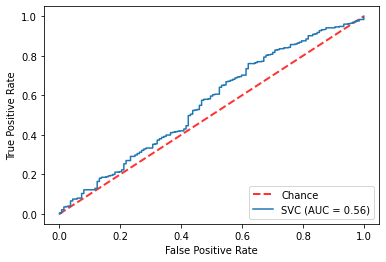
\includegraphics[scale=0.55]{images/base-de-dados-28.3.4-roc-curve-svc-monthly-cnae.png}
        \caption{Curva ROC para SVC}
        \label{fig:resultados:base-de-dados-28.3.4-roc-curve-svc-monthly-cnae}
    \end{subfigure}
    \fdadospesquisa
\end{figure}

\begin{figure}[htb] 
    \centering 
    \caption{Resultado das tentativas de classificação para cada método aplicado sobre dados de CNAEs para impacto total}
    \label{fig:resultados:classification-total-cnae} 
    \begin{subfigure}[b]{0.45\textwidth}
        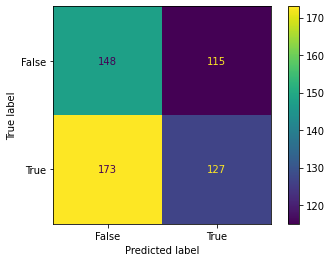
\includegraphics[scale=0.55]{images/base-de-dados-28.4.5-confusion-matrix-knn-total-cnae.png}
        \caption{Matriz de confusão para KNN}
        \label{fig:resultados:base-de-dados-28.3.5-confusion-matrix-knn-total-cnae}
    \end{subfigure} ~ \quad
    \begin{subfigure}[b]{0.45\textwidth}
        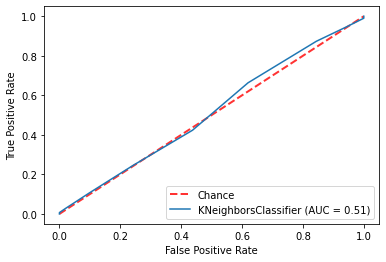
\includegraphics[scale=0.55]{images/base-de-dados-28.4.6-roc-curve-knn-total-cnae.png}
        \caption{Curva ROC para KNN}
        \label{fig:resultados:base-de-dados-28.3.6-roc-curve-knn-total-cnae}
    \end{subfigure} ~ \\
    \begin{subfigure}[b]{0.45\textwidth}
        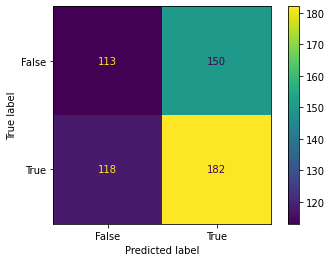
\includegraphics[scale=0.55]{images/base-de-dados-28.4.1-confusion-matrix-randomforest-total-cnae.png}
        \caption{Matriz de confusão para Random Forest}
        \label{fig:resultadosbase-de-dados-28.3.1-confusion-matrix-randomforest-total-cnae}
    \end{subfigure} ~ \quad
    \begin{subfigure}[b]{0.45\textwidth}
        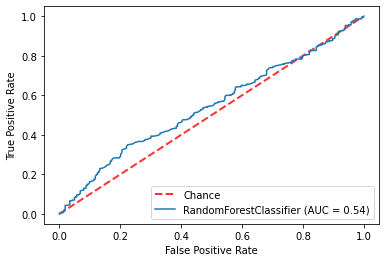
\includegraphics[scale=0.55]{images/base-de-dados-28.4.2-roc-curve-randomforest-total-cnae.png}
        \caption{Curva ROC para Random Forest}
        \label{fig:resultados:base-de-dados-28.3.2-roc-curve-randomforest-total-cnae}
    \end{subfigure} ~ \\
    \begin{subfigure}[b]{0.45\textwidth}
        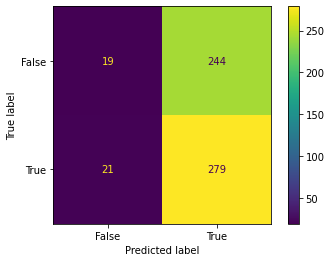
\includegraphics[scale=0.55]{images/base-de-dados-28.4.7-confusion-matrix-logregression-total-cnae.png}
        \caption{Matriz de confusão para Regressão logística}
        \label{fig:resultados:base-de-dados-28.3.7-confusion-matrix-logregression-total-cnae}
    \end{subfigure} ~ \quad
    \begin{subfigure}[b]{0.45\textwidth}
        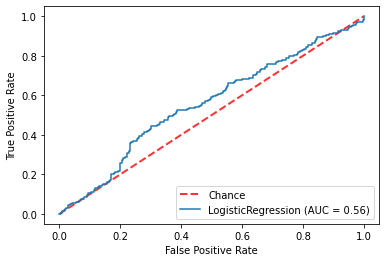
\includegraphics[scale=0.55]{images/base-de-dados-28.4.8-roc-curve-logregression-total-cnae.png}
        \caption{Curva ROC para Regressão Logística}
        \label{fig:resultados:base-de-dados-28.3.8-roc-curve-logregression-total-cnae}
    \end{subfigure} ~ \\
    \begin{subfigure}[b]{0.45\textwidth}
        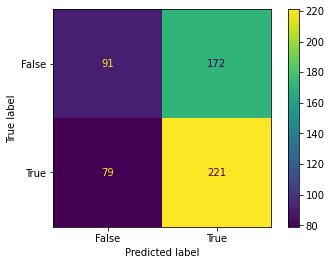
\includegraphics[scale=0.55]{images/base-de-dados-28.4.3-confusion-matrix-svc-total-cnae.png}
        \caption{Matriz de confusão para SVC}
        \label{fig:resultados:base-de-dados-28.3.3-confusion-matrix-svc-total-cnae}
    \end{subfigure} ~ \quad
    \begin{subfigure}[b]{0.45\textwidth}
        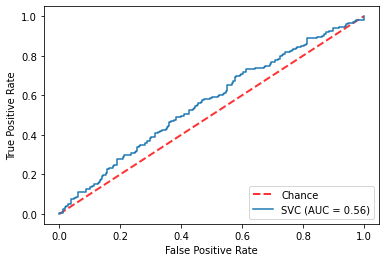
\includegraphics[scale=0.55]{images/base-de-dados-28.4.4-roc-curve-svc-total-cnae.png}
        \caption{Curva ROC para SVC}
        \label{fig:resultados:base-de-dados-28.3.4-roc-curve-svc-total-cnae}
    \end{subfigure} ~ \\
    \fdadospesquisa
\end{figure}

\subsection{Conclusões}
\label{section:deteccao-impacto:conclusoes}

Nesta seção, montamos uma tentativa de classificação de entidades impactadas e não impactadas pela crise causada pela pandemia. Foram utilizadas três abordagens, por UF, por seção, e por CNAE, e fizemos um estudo da variância e de como os dados se espalham.

Já na análise de componentes principais, foi possível perceber para os três conjuntos de dados que eles não possuem um espalhamento adequado para que um classificador esteja apto a separar os conjuntos de dados. Sendo que os classificadores escolhidos foram utilizados justamente para tentar utilizar diferentes abordagens de classificação.

Foram utilizadas também algumas técnicas para tentar reduzir o \textit{overfitting} nos dados: utilizamos a análise de componentes principais para selecionar apenas dimensões de maior taxa de explicabilidade, utilizamos técnicas de discretização dos dados para tentar uma melhor separação dos dados, e algumas variáveis não apresentadas aqui também foram inseridas no conjunto de dados e depois removidas ou por ser redundante com alguma outra variável, ou por ser insuficiente para um melhor espalhamento dos dados.

O resultado aqui obtido não o ideal, mas de forma alguma eles significam que seja impossível fazer um classificador que esteja apto a esses conjuntos de dados. Outros classificadores não utilizados aqui podem ter a capacidade de obter melhores resultados, e até mesmo os classificadores que foram utilizados podem apresentar resultados melhores com outros tratamentos aplicados aos dados ou com a adição de novas variáveis.
